%%
%% Arquivo principal adaptado para:
%% - Trabalho de Conclusão de Curso de Graduação - Eng. Computação e Mecatrônica - UFRN
%%
%% NOTA: A PUBLICAÇÃO DESTE MODELO VISA APENAS ORIENTAR OS PÓS-GRADUANDOS
%% NA PREPARAÇÃO DE SEUS TEXTOS. O PPgEE DA UFRN NÃO PROVÊ ASSISTÊNCIA NO
%% USO DAS FERRAMENTAS NECESSÁRIAS AO USO DESTE MODELO (LATEX, XFIG, ETC.)
%%
%% Baseado no modelo prévio para Tese de Pós Graduação PPGEEC do Prof. Dr.Adelardo Medeiros, dezembro de 2005.
%% Revisado pelos alunos de Metodologia da Pesquisa Científica de 2016.1.


%% -------------------------------------------------------------------------
%%
%% NOTA: Modelo adaptado em Julho de 2022 para template de TCC em Eng. de Computação 
%% e Mecatrônica da UFRN/CT.
%%
%% Válber César Cavalcanti Roza (Sec. de Coordenação de Eng.Mecatrônica CTEC/UFRN),20 de Julho, 2022.
%% Revisado pelo secretariado das Coordenações dos respectivos cursos.
%%
%% -------------------------------------------------------------------------


% DEFINIÇÕES GLOBAIS

% Esta primeira linha dá informações gerais sobre o documento.
% PARA A VERSÃO FINAL:
% papel A4, letra grande (12pt), openright (capítulos só iniciam em
% página direita, se necessário incluindo uma página em branco),
% twoside (o documento vai ser impresso em frente e costa)
\documentclass[a4paper,12pt,openright,twoside]{book}
% PARA A QUALIFICAÇÃO E PARA A VERSÃO INICIAL:
% papel A4, letra grande (12pt), openany (capítulos iniciam em
% qualquer página), oneside (o documento vai ser impresso só na frente)
%\documentclass[a4paper,12pt,openany,oneside]{book}


% Use estes pacotes para poder digitar diretamente as letras com acento
% e para que a hifenização funcione corretamente
\usepackage[utf8]{inputenc}
\usepackage{ae}
% Para usar fontes standard ao invés das do LaTeX (gera melhores PDFs)
\usepackage{pslatex}
% Para a hifenização em português
\usepackage[portuges, brazil]{babel}
% Para que os primeiros parágrafos das seções também sejam indentados
\usepackage{indentfirst}
% Para poder incluir gráficos (figuras)
\usepackage{graphicx}
\usepackage{subfig}
% Para poder fazer glossário ou lista de símbolos
% Use a segunda opção se quiser incluir na definição do símbolo a
% página e/ou a equação onde ela foi definida
\usepackage[portuguese,noprefix]{nomencl}
%\usepackage[portuguese,noprefix,refeq,refpage]{nomencl}
% Para permitir espaçamento simples, 1 1/2 e duplo
\usepackage{setspace}
% Para usar alguns comandos matemáticos avançados muito úteis
\usepackage{amsmath}
% Para poder usar o ambiente "comment"
\usepackage{verbatim}
% Para poder ter tabelas com colunas de largura auto-ajustável
\usepackage{tabularx}
% Para executar um comando depois do fim da página corrente
\usepackage{afterpage}
% Para formatar URLs (endereços da Web)
\usepackage{url}
% Para reduzir os espaços entre os itens (itemize, enumerate, etc.)
% Este pacote não faz parte da distribuição padrão do LaTeX.
\usepackage{lib/noitemsep}
% Para as citações bibliográficas
%\usepackage[alf]{abntex2cite}
\usepackage[abbr]{lib/harvard}	% As chamadas são sempre abreviadas
%\harvardparenthesis{square}	% Colchetes nas chamadas
%\harvardyearparenthesis{round}	% Parêntesis nos anos das referências
%\renewcommand{\harvardand}{e}	% Substituir "&" por "e" nas referências

% PACOTES OPCIONAIS
\usepackage[table, xcdraw]{xcolor}
\usepackage{hhline} % https://tex.stackexchange.com/questions/121476/table-cell-color-overlaps-cell-border
% Para poder incluir arquivos Postscript com cores (do Xfig, por exemplo)
\usepackage{color, colortbl}
% Para ter células em tabelas que ocupam mais de uma linha
\usepackage{multirow}
% Para poder ter tabelas longas em mais de uma página
\usepackage{longtable}
% Para poder escrever partes do texto em "n" colunas
%\usepackage{multicol}
% Se você quiser personalizar os cabeçalhos das páginas
%\usepackage{fancyheadings}
% Para incluir algoritmos e listagens de códigos
\usepackage{listings}
% Para incluir pseudocódigos
\usepackage[portuguese, ruled, linesnumbered]{algorithm2e}
% Capítulos com títulos em um formato "decorado"
\usepackage{lib/capitulos}
% Hiper-referências dentro do texto e montagem dos links do índices dos
% para os leitores de pdf (deve ser o último pacote a ser inserido).
\usepackage[breaklinks]{hyperref}
% Referência correta de ambientes flutuantes (como figuras, tabelas e algoritmos).
\usepackage[all]{hypcap}
\usepackage{titlesec}
\usepackage{enumitem}

% NOVOS COMANDOS

% As definições dos novos comandos estão agrupadas no arquivo "comandos.tex"
% Esta separação é opcional: se você preferir, pode por as definições
% diretamente neste arquivo
% newcommand define novos comandos, que podem passar a ser usados da
% mesma forma que os comandos LaTeX de base.

% Implicação em fórmulas
\newcommand{\implica}{\quad\Rightarrow\quad} %Meio de linha
\newcommand{\implicafim}{\quad\Rightarrow}   %Fim de linha
\newcommand{\tende}{\rightarrow}
\newcommand{\BibTeX}{\textsc{B\hspace{-0.1em}i\hspace{-0.1em}b\hspace{-0.3em}}\TeX}

% Fração com parentesis
\newcommand{\pfrac}[2]{\left(\frac{#1}{#2}\right)}

% Transformada de Laplace e transformada Z
%\newcommand{\lapl}{\makebox[0cm][l]{\hspace{0.1em}\raisebox{0.25ex}{-}}\mathcal{L}}
\newcommand{\lapl}{\pounds}
\newcommand{\transfz}{\mathcal{Z}}

% Não aparecer o número na primeira página dos capítulos
\newcommand{\mychapter}[1]{\chapter{#1}\thispagestyle{empty}}

% Os capítulos sem número
\newcommand{\mychapterast}[1]{\chapter*{#1}\thispagestyle{empty}
\chaptermark{#1}
\afterpage{\markboth{\uppercase{#1}}{\rightmark}}
\markboth{\uppercase{#1}}{}
}

% Seções sem número
\newcommand{\mysectionast}[1]{\section*{#1}
\addcontentsline{toc}{section}{#1}
\markright{\uppercase{#1}}
}

% No tabularx, as celulas devem ser centradas verticalmente
\renewcommand{\tabularxcolumn}[1]{m{#1}}

% Células centralizadas horizontalmente no tabularx
\newcolumntype{C}{>{\centering\arraybackslash}X}

%% Abrevia figuras e tabelas
%\def\figurename{Fig.}
%\def\tablename{Tab.}

% Created by Leonardo Rignanese (rignaneseleo)
% https://github.com/rignaneseleo/Latex-listings-Dart

\usepackage{xcolor}

% Define colors to use
% You can change the colors (use http://latexcolor.com/)
\definecolor{white}{rgb}{1,1,1}
\definecolor{codegreen}{rgb}{0,0.6,0}
\definecolor{codeblue}{rgb}{0.14,0.41,0.64}
\definecolor{codeligthblue}{rgb}{0.51,0.76,0.9}
\definecolor{codegray}{rgb}{0.5,0.5,0.5}
\definecolor{codepurple}{rgb}{0.58,0,0.82}
\definecolor{amber(sae/ece)}{rgb}{1.0, 0.49, 0.0}
% \definecolor{backcolour}{rgb}{0, 0, 0}
\definecolor{backcolour}{rgb}{0.95, 0.95, 0.96}
% \definecolor{backcolour}{rgb}{0.12, 0.12, 0.12}
% \definecolor{backcolour}{rgb}{0.22, 0.22, 0.22}
\definecolor{unitednationsblue}{rgb}{0.36, 0.57, 0.9}

\renewcommand{\lstlistingname}{Código}% Listing -> Código
\renewcommand{\lstlistlistingname}{Lista de \lstlistingname s}% List of Listings -> List of Códigos

% Define the codebox
\lstset{
backgroundcolor=\color{backcolour},   
    commentstyle=\color{codegreen},
    keywordstyle=\color{magenta},
    numberstyle=\tiny\color{codegray},
    stringstyle=\color{codepurple},
    basicstyle=\ttfamily\footnotesize,
    breakatwhitespace=false,         
    breaklines=true,                 
    captionpos=b,                    
    keepspaces=true,                 
    numbers=left,                    
    numbersep=5pt,                  
    showspaces=false,                
    showstringspaces=false,
    showtabs=false,                  
    tabsize=2,
    % frame=shadowbox
}   

% Define the code emph rules
\lstset{
    %%%%%%%%%%%%%%%%%%%%%%%%%%%%
    %%%%%%%%%% Types %%%%%%%%%%%
    %%%%%%%%%%%%%%%%%%%%%%%%%%%%
    emph=
    {   % Cada linha a partir da segunda é de um código existente
        var, String, int, List, dynamic %
        BotaoPrincipal, StatelessWidget, Key, Widget, BuildContext, TextButton, Text, %
        CampoTexto, State, CampoTextoState, _CampoTextoState, TextField, InputDecoration, %
        GenericModel, Map, %
        CampaignRepository, Campaign, %
        AddCampaignFormController, AddFormController, %
        DatabaseCampaignRepository, DatabaseInterface, DatabaseManager, %
        HomeController, ApplicationRepository, ObservableList, Application, Action, DatabaseApplicationRepository, Future, %
        Home, Scaffold, VaccinationButton, %
        Appliers, Provider, AppliersPageController, EntityList, Applier, %
        Vaccine, Validator, ValidatorType, ValidationPair, %
        DateTime, %
    },
    emphstyle=\color{codegreen},
    %%%%%%%%%%%%%%%%%%%%%%%%%%%%
    %%%%%%%%% Functions %%%%%%%%
    %%%%%%%%%%%%%%%%%%%%%%%%%%%%
    emph=
    { % Cada linha é de um código existente
        [2]build, print, setState, createState, %
        toMap, %
        createCampaign, deleteCampaign, getCampaignById, getCampaignByTitle, getCampaigns, updateCampaign, %
        create, delete, %
        of, empty, getApplications, clear, addAll, %
        read, %
        trim, _validateVaccine, validate, validateAll, %
        main, setUp, group, test, expect, isA, %
    },
    emphstyle={[2]\color{magenta}},
    %%%%%%%%%%%%%%%%%%%%%%%%%%%%
    %%%%%%%%% Keywords %%%%%%%%%
    %%%%%%%%%%%%%%%%%%%%%%%%%%%%
    emph={[3]class, extends, final, const, required, super, this, late, true, null, abstract, implements, static, void},
    emphstyle={[3]\color{codeblue}},
    %%%%%%%%%%%%%%%%%%%%%%%%%%%%
    %%%%%%%% Keywords 2 %%%%%%%%
    %%%%%%%%%%%%%%%%%%%%%%%%%%%%
    emph={[4]return, async, await},
    emphstyle={[4]\color{codepurple}},
    %%%%%%%%%%%%%%%%%%%%%%%%%%%%
    %%%%%%%%% Strings %%%%%%%%%%
    %%%%%%%%%%%%%%%%%%%%%%%%%%%%
    emph=
    {
        [5]", Clicou, no, botao, principal, %
        Digite, aqui, %
        vaccinations, new, %
        Aplicantes, %
        Title, Description, criacao, de, nova, instancia, de, campanha, deve, criar, uma, valida, %
    },
    emphstyle={[5]\color{amber(sae/ece)}},
    %%%%%%%%%%%%%%%%%%%%%%%%%%%%
    %%%%%%%% Variables %%%%%%%%%
    %%%%%%%%%%%%%%%%%%%%%%%%%%%%
    emph=
    {   % Cada linha é de um código existente
        [6]texto, key, override, context, onPressed, child, %
        onChanged, value, decoration, labelText, widget, hintText, %
        campaign, %
        _repository, campaignRepository, %
        TABLE, dbManager, count, %
        applicationRepository, applications, growable, fetchApplications, result, reversed, %
        floatingActionButton, newPage, onCallback, %
        controller, title, %
        id, sipniCode, name, laboratory, numericalString, %
        validCampaign, description, startDate, endDate, %
    },
    emphstyle={[6]\color{codeligthblue}}%
}


%
% As margens
%

% Direção horizontal

% Margem interna
% Nas páginas ímpares
\setlength{\oddsidemargin}{3.5cm}         % Margem real desejada
% Nas páginas pares
\setlength{\evensidemargin}{2.5cm}        % Margem real desejada
% Largura do texto
\setlength{\textwidth}{15cm}
% As margens laterais no LaTeX são sempre 1 polegada maiores do que as
% fixadas. Se foi fixada \setlength{\oddsidemargin}{3.5cm}, a margem
% real seria de 3.5+2.54=6.04cm. Para permitir que você não tenha que
% fazer esta conta, pode usar o número desejado nas linhas anteriores
% e a gente subtrai 1in nas próximas linhas
\addtolength{\oddsidemargin}{-1in}
\addtolength{\evensidemargin}{-1in}
% Note que a margem direita não é fixada diretamente:
% ela é obtida subtraindo-se os outros valores da largura da página.
% 3.5+15+x=21cm (largura A4) -> x = margem externa = 2.5cm

% Direção vertical

% Margem superior (entre o topo da folha e o cabeçalho), altura do
% cabeçalho e distância entre o fim do cabeçalho e o início do texto
\setlength{\topmargin}{2.0cm}             % Margem real desejada
\setlength{\headheight}{1.0cm}
\setlength{\headsep}{1.0cm}
% Altura do texto (sem cabeçalho e rodapé)
\setlength{\textheight}{22.7cm}
% Distância do fim do texto ao rodapé
\setlength{\footskip}{1.0cm}
% A margem superior no LaTeX é sempre 1 polegada maior do que a
% fixada. Se foi fixada \setlength{\topmargin}{2.0cm}, a margem
%real seria de 2.0+2.54=4.54cm. Para permitir que você não tenha que
% fazer esta conta, pode usar o número desejado na linha anterior
% e a gente subtrai 1in na próxima linha
\addtolength{\topmargin}{-1in}
% Note que a margem inferior não é fixada diretamente:
% ela é obtida subtraindo-se os outros valores, sem incluir o
% "footskip", da altura da página.
% 2.0+1.0+1.0+22.7+x=29.7cm (altura A4) -> x = margem inferior = 3cm

%
% O estilo das referências bibliográficas
%

\bibliographystyle{bibliografia/ppgee}

%
% O espaçamento entre linhas
%

% As páginas iniciais são sempre em espaçamento simples
\singlespacing

% Para a criação do glossário (ou lista de símbolos)
\makenomenclature

% Lista de arquivos a serem processados. Estes comandos "includeonly" são
% dispensáveis e devem obrigatoriamente ser comentados na hora de gerar o
% documento definitivo. Eles servem para compilar apenas parte do documento.
% É útil, durante a redação, para que não se tenha de compilar todo o
% documento a cada vez que se faz uma alteração. Por exemplo, se eu estou
% fazendo alterações na dedicatória e as outras partes não têm interesse no
% momento, posso incluir (descomentar) a linha "\includeonly{preambulo}"
%\includeonly{rosto}
%\includeonly{catalograficos}
%\includeonly{preambulo}
%\includeonly{resumos}
%\includeonly{textuais/cap1_introducao.tex}
% \includeonly{textuais/cap2_teoria}
% \includeonly{textuais/cap3_trabalhos_relacionados.tex}
% \includeonly{textuais/cap4_implementacao.tex}
% \includeonly{textuais/cap5_experimentos_e_resultados.tex}
% \includeonly{textuais/cap6_conclusao.tex}
%\includeonly{estilo/estilo}
%\includeonly{matematica/matematica}
%\includeonly{figuras/figuras}
%\includeonly{conclusao/conclusao}
%\includeonly{apendice/apendice}

\setlength{\arrayrulewidth}{0.5mm}
\renewcommand{\arraystretch}{2}

% Inicia o texto
\begin{document}

% Paginas iniciais (sem numeração)
\pagestyle{empty}

% Página de rosto (capa interna)
%
% ********** Página de Rosto
%

% titlepage gera páginas sem numeração
\begin{titlepage}

\begin{center}

\small

\begin{tabularx}{\linewidth}{@{}l@{}C@{}r@{}}
\parbox[c]{3cm}{
\includegraphics[width=\linewidth]{./figuras/UFRN}} &
\begin{center}
\textsf{\textsc{Universidade Federal do Rio Grande do Norte\\
Centro de Tecnologia\\
Graduação em Engenharia de Computação}}
\end{center} &
\parbox[c]{3cm}{
\includegraphics[width=\linewidth]{./figuras/dca_logo.png}}
\end{tabularx}

\vfill
\LARGE
\textbf{Nurse}
\vfill
\Large
\textbf{Dorgival da Rocha Filho}
\vfill

\normalsize

Orientador: Prof. Dr. Severino Lampeão
\\[2ex] Co-orientador: Prof. Dr. Zé Baiano % Opcional

\vfill

\hfill


\vfill

\large

Natal, RN, \today

\end{center}

\end{titlepage}

% Página de rosto (capa interna)
%
% ********** Página de Rosto
%

% titlepage gera páginas sem numeração
\begin{titlepage}

\begin{center}

\small

\begin{tabularx}{\linewidth}{@{}l@{}C@{}r@{}}
\parbox[c]{3cm}{
\includegraphics[width=\linewidth]{./figuras/UFRN}} &
\begin{center}
\textsf{\textsc{Universidade Federal do Rio Grande do Norte\\
Centro de Tecnologia\\
Graduação em Engenharia de Computação}}
\end{center} &
\parbox[c]{3cm}{
\includegraphics[width=\linewidth]{./figuras/dca_logo.png}}
\end{tabularx}

\vfill
\LARGE
\textbf{Nurse: aplicação mobile para controle dos dados de vacinação e aumento de produtividade de profissionais da saúde}
\vfill
\Large
\textbf{Dorgival da Rocha Filho}
\vfill

\normalsize

Orientador: Prof. Dr. Itamir de Morais Barroca Filho

\vfill

\hfill
\parbox{0.5\linewidth}{\textbf{%
Trabalho de Conclusão de Curso de Graduação} na modalidade Monografia, 
submetido como parte dos requisitos necessários para 
conclusão do curso de Engenharia de Computação pela 
Universidade Federal do Rio Grande do Norte (UFRN/CT).
}

\vfill

\large

Natal, RN, \today

\end{center}

\end{titlepage}


% Ficha catalográfica: os dados catalográficos devem ser fornecidos
% pela BCZM.
% Só são incluídos na versão final da tese ou dissertação. Não são
% incluídos nem na proposta de tema de qualificação nem na versão
% preliminar da tese ou dissertação: nestes casos, comente a próxima linha.
% %
% ********** Ficha Catalográfica
%

\newpage

\begin{center}
  % Aqui não se usou \vfill porque o \vfill é construído internamente com
  % o comando \vspace. Espaços verticais no início da folha com \vspace
  % são ignorados. Para que isto não ocorra deve-se usar o \vspace*
  % \vspace*{\fill} é como se fosse um \vfill*
  \vspace*{\fill}
  \fontsize{10}{12}\selectfont
  
  \textsf{Universidade Federal do Rio Grande do Norte - UFRN \\
  Sistema de Bibliotecas - SISBI \\
  Catalogação de Publicação na Fonte. UFRN - Biblioteca Central Zila Mamede}
  
  \vspace{2ex}
  
  \begin{minipage}[c]{12.5cm}
    \begin{tabular}{|p{\linewidth}|} \hline \texttt{Rocha Filho, Dorgival da.} \linebreak
    \texttt{\hspace*{1em} Nurse: aplicação mobile para controle dos dados de vacinação \linebreak
    e aumento de produtividade de profissionais da saúde / Dorgival \linebreak
    da Rocha Filho -- Natal, 2022.} \linebreak
    \hspace*{1em} \texttt{88 f.: il}
    \\[1ex]
    \texttt{\hspace{1em} Monografia (graduação) - Universidade Federal do Rio Grande \linebreak
    do Norte, Centro de Tecnologia, Curso de Engenharia de \linebreak Computação.} \linebreak
    \hspace*{1em} \texttt{Orientador: Prof. Dr. Itamir de Morais Barroca Filho.}
    \\[3ex]
    \texttt{\hspace{1em} 1. Framework Flutter - Monografia. 2. Vacinação - Monografia. \linebreak 3. Aplicação Móvel - Monografia.
    I. Barroca Filho, Itamir de \linebreak Morais.
    II. Título.}
    \\
    \texttt{RN/UF/BCZM} \hfill \texttt{CDU 004.4:614.47} \hspace{3cm} \\
    \\
    \hline
    \end{tabular} 
    \\[3ex]
    \texttt{Elaborado por Fernanda de Medeiros Ferreira Aquino - CRB-15/301}
  \normalsize
  \end{minipage}
\end{center}
\vspace{4cm}


% Assinaturas da banca, dedicatória e agradecimentos
% Só são incluídos na versão final da tese ou dissertação. Não são
% incluídos nem na proposta de tema de qualificação nem na versão
% preliminar da tese ou dissertação: nestes casos, comente a próxima linha.
% %
% ********** Página de assinaturas
%

\begin{titlepage}

\begin{center}

\LARGE

\textbf{Nurse: aplicação mobile para controle dos dados de vacinação e aumento de produtividade de profissionais da saúde}

\vfill

\Large

\textbf{Dorgival da Rocha Filho}

\end{center}

\vfill

% O \noindent é para eliminar a tabulação inicial que normalmente é
% colocada na primeira frase dos parágrafos
\noindent
% Descomente a opção que se aplica ao seu caso
% Note que propostas de tema de qualificação nunca têm preâmbulo.
Monografia aprovada em 09 de dezembro de 2022, pela banca examinadora composta
pelos seguintes membros:

% Os nomes dos membros da banca examinadora devem ser listados
% na seguinte ordem: orientador, co-orientador (caso haja),
% examinadores externos, examinadores internos. Dentro de uma mesma
% categoria, por ordem alfabética

\begin{center}

\vspace{1.5cm}\rule{0.95\linewidth}{1pt}
\parbox{0.9\linewidth}{%
Prof. Dr. Itamir de Morais Barroca Filho (orientador) \dotfill\ DTI-IMD/UFRN}

% \vspace{1.5cm}\rule{0.95\linewidth}{1pt}
% \parbox{0.9\linewidth}{%
% Prof. Dr. YYYYY (co-orientador) \dotfill\ MCA/UFRN}

\vspace{1.5cm}\rule{0.95\linewidth}{1pt}
\parbox{0.9\linewidth}{%
Prof. Dr. André Morais Gurgel \dotfill\ DEPAD/CCSA/UFRN}

\vspace{1.5cm}\rule{0.95\linewidth}{1pt}
\parbox{0.9\linewidth}{%
Prof. Dr. Jean Mário Moreira de Lima \dotfill\ IMD/UFRN}

\end{center}

\end{titlepage}

%
% ********** Dedicatória
%

% A dedicatória não é obrigatória. Se você tem alguém ou algo que teve
% uma importância fundamental ao longo do seu curso, pode dedicar a ele(a)
% este trabalho. Geralmente não se faz dedicatória a várias pessoas: para
% isso existe a seção de agradecimentos.
% Se não quiser dedicatória, basta excluir o texto entre
% \begin{titlepage} e \end{titlepage}

\begin{titlepage}

\vspace*{\fill}

\hfill
\begin{minipage}{0.5\linewidth}
\begin{flushright}
\large\it
Aos meus ......
\end{flushright}
\end{minipage}

\vspace*{\fill}

\end{titlepage}

%
% ********** Agradecimentos
%

% Os agradecimentos não são obrigatórios. Se existem pessoas que lhe
% ajudaram ao longo do seu curso, pode incluir um agradecimento.
% Se não quiser agradecimentos, basta excluir o texto após \chapter*{...}

\chapter*{Agradecimentos}
\thispagestyle{empty}

\begin{trivlist}  \itemsep 2ex

\item Ao meu orientador e ao meu co-orientador, professores XXXXXX e YYYYYY, sou grato pela orientação.

\item Ao secretário Halidaivson Stockhouse pela ajuda no andamento das coisas burocráticas do Curso.

\item Aos colegas ....

\item Aos demais colegas de graduação, pelas críticas e sugestões.

\item À minha família pelo apoio durante esta jornada.

\item À CAPES/CNPQ, pelo apoio financeiro.

\item À Deus.

\end{trivlist}


%
% O espaçamento entre linhas (ATENÇÃO A ESTA PARTE!)
%
%%%%%%%%%%%%%%%%%%%%%%%%%%%%%%%%%%%%%%%%%%%%%%%%%%%%%%%%%%%%%%%%%%%%%%%%%%%%
% PARA A VERSÃO FINAL:
% Deve ser usado espaçamento simples nas páginas de texto
% \singlespacing
% PARA A QUALIFICAÇÃO E PARA A VERSÃO INICIAL:
% Deve ser usado espaçamento 1 1/2 nas páginas de texto
\doublespacing
%%%%%%%%%%%%%%%%%%%%%%%%%%%%%%%%%%%%%%%%%%%%%%%%%%%%%%%%%%%%%%%%%%%%%%%%%%%%

% Resumo/Abstract
%
% ********** Resumo
%

% Usa-se \chapter*, e não \chapter, porque este "capítulo" não deve
% ser numerado.
% Na maioria das vezes, ao invés dos comandos LaTeX \chapter e \chapter*,
% deve-se usar as nossas versões definidas no arquivo comandos.tex,
% \mychapter e \mychapterast. Isto porque os comandos LaTeX têm um erro
% que faz com que eles sempre coloquem o número da página no rodapé na
% primeira página do capítulo, mesmo que o estilo que estejamos usando
% para numeração seja outro.
\mychapterast{Resumo}

Lorem ipsum dolor sit amet, consectetur adipiscing elit. Donec vehicula vitae lectus ut pretium. Vestibulum tristique leo eu purus vehicula ullamcorper. Nulla ut ultricies massa. Suspendisse eu neque pharetra, faucibus erat ac, pretium augue. Vivamus id euismod leo. Cras eget neque pellentesque, fringilla dolor eu, pretium libero. Mauris sed justo feugiat, varius ligula sed, posuere metus. Fusce lacus mi, molestie a rutrum id, scelerisque ut lacus. In hac habitasse platea dictumst. In vitae elit faucibus, molestie orci efficitur, consectetur neque. Ut placerat, augue eu pellentesque euismod, dui enim euismod elit, quis sollicitudin lectus lorem gravida mi. Donec ut leo pretium, finibus arcu in, tincidunt sem. Phasellus diam ante, pulvinar vel neque non, sagittis aliquam nibh. Praesent id condimentum nunc, quis interdum metus. Curabitur eget diam vitae enim consequat mollis quis dictum turpis.

\vspace{1.5ex}

{\bf Palavras-chave}: Processamento de texto, \LaTeX,
Preparação de Teses, Relatórios Técnicos.

%
% ********** Abstract
%
\mychapterast{Abstract}

Lorem ipsum dolor sit amet, consectetur adipiscing elit. Donec vehicula vitae lectus ut pretium. Vestibulum tristique leo eu purus vehicula ullamcorper. Nulla ut ultricies massa. Suspendisse eu neque pharetra, faucibus erat ac, pretium augue. Vivamus id euismod leo. Cras eget neque pellentesque, fringilla dolor eu, pretium libero. Mauris sed justo feugiat, varius ligula sed, posuere metus. Fusce lacus mi, molestie a rutrum id, scelerisque ut lacus. In hac habitasse platea dictumst. In vitae elit faucibus, molestie orci efficitur, consectetur neque. Ut placerat, augue eu pellentesque euismod, dui enim euismod elit, quis sollicitudin lectus lorem gravida mi. Donec ut leo pretium, finibus arcu in, tincidunt sem. Phasellus diam ante, pulvinar vel neque non, sagittis aliquam nibh. Praesent id condimentum nunc, quis interdum metus. Curabitur eget diam vitae enim consequat mollis quis dictum turpis.

\vspace{1.5ex}

{\bf Keywords}: Document Processing, \LaTeX, Thesis Preparation,
Technical Reports.


% Paginas introdutórias (com numeração romana)
\frontmatter

% Lista de conteúdo (sumário, gerado automaticamente)
% Aqui, e em todos os itens antes da introdução, o comando \phantomsection é utilizado.
% O seu uso é necessário para auxiliar o pacote "hyperref" a fazer a referência correta
% dos links do sumário, das listas (de tabelas, figuras, algoritmos) com as páginas
% respectivas.
% Caso seja tirado, o "hyperref" irá apontar o link do sumário para o abstract, o link
% do sumário para a lista de figuras, o link das listas de figuras para a lista de tabelas,
% e assim sucessivamente.
\phantomsection
\addcontentsline{toc}{chapter}{Sumário}
\tableofcontents

% Lista de figuras (gerada automaticamente)
\cleardoublepage
\phantomsection
\addcontentsline{toc}{chapter}{Lista de Figuras}
\listoffigures

% Lista de tabelas (gerada automaticamente)
\cleardoublepage
\phantomsection
\addcontentsline{toc}{chapter}{Lista de Tabelas}
\listoftables

% Lista de códigos (gerada automaticamente)
\cleardoublepage
\phantomsection
\addcontentsline{toc}{chapter}{Lista de Códigos}
\lstlistoflistings

% Lista de abreviações 
\cleardoublepage
\phantomsection
\addcontentsline{toc}{chapter}{Lista de Abreviaturas e Siglas}
\mychapterast{Lista de Abreviaturas e Siglas}

\begin{center}
  \begin{tabularx}{\textwidth}{
    >{\raggedright\arraybackslash}m{0.10\textwidth} 
    >{\raggedright\arraybackslash}X }
    CNES & Cadastro Nacional de Estabelecimentos de Saúde \\
    CNS  & Cadastro Nacional de Saúde \\
    CPF  & Cadastro de Pessoa Física \\
    SARS & Síndrome Aguda Respiratória Grave \\
    SUS  & Sistema Único de Saúde \\
  \end{tabularx}
  \label{tab:abbr}
\end{center}


% Páginas do texto principal (com cabeçalho)
\mainmatter
\pagestyle{headings}

% Para facilitar a organização, foi criado um diretório para cada
% capítulo do documento, pois assim os arquivos das figuras ficam
% classificados por capítulos

% Cap. 1 - Introdução
%%
%% Capítulo 1: Introdução
%%

\mychapter{Introdução}
\label{Cap:Introducao}
% Dicas para o trabalho
% [A revisar] Fazer uma ou duas perguntas relacionadas ao trabalho que serão respondidas no decorrer do mesmo.
% O objeto do projeto é tornar o registro de dados sobre a vacinação contra a COVID-19 mais fácil e rápido para os profissionais de saúde, de forma que possam se concentrar em outras atividades. Esse registro é feito manualmente e em papel, o que pode gerar erros e atrasos no processo de cadastro. O objetivo do projeto é criar um sistema que organize os dados e envio-os por meio de planilhas que poderão ser enviadas ao sistema único de saúde.

% [A fazer] Escrever por que essa solução deve ser usada e qual o problema ele resolve.

% [As informações de Titita] Existem dois sistemas para informação das vacinações do município: esus pec e o novo sipni.
% O manual de vacinação
% O velho sipni (sipni web) era usado paras campanhas de vacinação contra influenza e poliomelite. Agora todas as campanhas são feitas no novo sipni. Nesse ano de 2022 já foram feitas campanhas contra sarampo, polio e influenza.

% Cada campanha tem um manual técnico/operacional. 


\section{Contextualização}
\label{cap1:Sec:Contextualizacao}
% [A revisar]
Em 2019 surgiu o vírus SARS-Cov-2, responsável por causar a maior pandemia já registrada na história, chamada Covid-19. Desde então, uma grande mobilização em todos os países começou visando a criação de uma vacina contra a doença causada pelo vírus e a consequente corrida para a sua produção em massa. De acordo com a Organização Mundial da Saúde (OMS), no início de 2021 existiam 236 vacinas candidatas em fases pré- clínicas ou fase clínica.
% ref.: Plano Nacional de Operacionalização da Vacinação contra a Covid-19 - PNO (2ª Edição com ISBN) 1. Introdução - https://www.gov.br/saude/pt-br/coronavirus/vacinas/plano-nacional-de-operacionalizacao-da-vacina-contra-a-covid-19

No Brasil, a vacinação contra a COVID-19 começou em 18 de janeiro de 2021, com a vacina Coronavac, produzida pelo Instituto Butantan em parceria com a farmacêutica chinesa Sinovac. A vacinação foi realizada em etapas, à medida em que as vacinas eram fabricadas e priorizando os grupos de maior risco de contaminação e de complicações da doença: profissionais da saúde, idosos, pessoas com comorbidade, pessoas com deficiência e população indígena. A vacinação foi feita em todo o país e com a utilização de um plano nacional, mas cada estado e município teve sua própria estratégia para a vacinação, em geral, pautada nesse plano.
% ref.: Plano Nacional de Operacionalização da Vacinação contra a Covid-19 - PNO (2ª Edição com ISBN) 3. População Alvo - https://www.gov.br/saude/pt-br/coronavirus/vacinas/plano-nacional-de-operacionalizacao-da-vacina-contra-a-covid-19


% [A revisar]
Independente da estratégia de vacinação de cada estado e em decorrência da necessidade de mapear com exatidão as pessoas que receberam a vacina, o Ministério da Saúde criou um módulo para o registro de dados nominais sobre a vacinação, o que inclui dados pessoais d(a) vacinado(a), e dose e lote administrados.

Esse sistema foi denominado Sistema de Informação de Programas de Imunização (Novo SI-PNI), e é usado para o registro de dados sobre as campanhas de vacinação. O SIPNI é um sistema web, que pode ser acessado pelo site da SES-SP, e é usado por profissionais de saúde para o registro de dados sobre a vacinação. O SIPNI é dividido em duas partes: o SIPNI Web e o SIPNI Mobile. O SIPNI Web é usado para o registro de dados sobre as campanhas de vacinação, e o SIPNI Mobile é usado para o registro de dados sobre a vacinação em campo.

% ref.: Plano Nacional de Operacionalização da Vacinação contra a Covid-19 - PNO (2ª Edição com ISBN) 3. População Alvo - https://www.gov.br/saude/pt-br/coronavirus/vacinas/plano-nacional-de-operacionalizacao-da-vacina-contra-a-covid-19

\section{Problema}
\label{cap1:Sec:Problema}
% Planilha de registro manual de vacinados. Essa imagem deve ser colocada para explicar como é feita a vacinação atualmente.
% Registro Manual de Vacinados - Conasems https://www.conasems.org.br 02/11/2022

% [A fazer] Tirar print da plataforma online de cadastro das vacinações
\subsection{Procedimento comum de vacinação}
\label{cap1:SubSec:cap1:ProcedimentoComumVacinacao}
O material de trabalho comumente utilizado é o papel com a planilha para preenchimento impressa. Feitas as anotações, esses dados são digitados em um sistema de cadastro de vacinação. Dessa forma, existe alguns pontos de falha no processo, como a possibilidade de erro de escrita da informação no momento da sua coleta ou de digitação, no momento em que esses dados são repassados para o sistema online; perda dos dados e dificuldade de compartilhamento dos mesmos.

% Ficha de vacinação: https://sisaps.saude.gov.br/esus/ ---> https://sisaps.saude.gov.br/esus/#:~:text=Manual%20PEC/CDS-,Fichas%20%2D%20CDS,-Fichas%20vigentes --->  http://189.28.128.100/dab/docs/portaldab/documentos/esus/ficha_vacinacao_COVID-19.pdf

% [A fazer] Adicionar imagem da planilha disponibilizada pelo governo para o registro escrito de vacinados
% [A fazer] Adicionar print da plataforma online de cadastro das vacinações

% [A analisar] Posso ir me perguntando vários porquês das coisas e colocar aqui para escrever sobre isso.

% [A analisar] Posso juntar trabalhos relacionados com problema em um mesmo capítulo.


% \begin{table}[htbp]
% \begin{tabularx}{\linewidth}{|p{3cm}|X|l|} \hline
% COLUNA p & COLUNA X & COLUNA l \\ \hline
% Largura fixa (não depende do conteúdo) &
% Expansível &
% Ajustável \\ \hline
% Alinhada no topo &
% Alinhada à esquerda &
% Alinhada à esquerda \\ \hline
% \end{tabularx}
% \\[0.5cm]
% \begin{tabularx}{\linewidth}{|b{3cm}|C|r|} \hline
% COLUNA b & COLUNA C (ver \texttt{comandos.tex}) & COLUNA r \\ \hline
% Largura fixa (não depende do conteúdo) &
% Expandível &
% Ajustável \\ \hline
% Alinhada na base &
% Centralizada &
% Alinhada à direita \\ \hline
% \end{tabularx}
% \caption{Tabelas com colunas de diferentes larguras e alinhamentos}
% \label{Tab:larguracolunas}
% \end{table}



\section{Objetivos}
\label{cap1:Sec:Objetivos}


\section{Estrutura do Trabalho}
\label{cap1:Sec:EstruturaTrabalho}



% Cap. 2 - Teoria (Fundamentação Teórica)
%%
%% Capítulo 2: Regras gerais de estilo
%%

\mychapter{Fundamentação Teórica}
\label{Cap:Teoria}

Neste capítulo serão apresentados os conceitos básicos relacionados ao \textit{framework Flutter}, assim como a linguagem de programação Dart, a biblioteca MobX e o \textit{wrapper} Provider, utilizados para o desenvolvimento desta aplicação.

Também serão discutidas as principais ideias relacionadas à Programação Orientada a Objeto (POO), aos bancos de dados relacionais e, por fim, alguns conceitos relacionados às boas práticas da programação no quesito de arquitetura de sistemas e os princípios SOLID.

\section{Dart}
\label{Sec:Dart}

Nessa seção, busca-se apresentar os conceitos básicos da linguagem Dart, utilizada para o desenvolvimento do \textit{framework} Flutter. O foco agora é mostrar as características que fizeram com que a linguagem Dart foi escolhida para ser a linguagem de programação do \textit{framework} Flutter.

\subsection{Introdução}
\label{SubSec: Introducao}

Dart é uma linguagem de programação criada pela Google em 2011, com o objetivo de ser utilizada, inicialmente, para o desenvolvimento de aplicações web, mas que tem como objetivo atual ser executada em qualquer plataforma.
% ref: http://googlecode.blogspot.com/2011/10/dart-language-for-structured-web.html 04/11/2022
% ref: https://dart.dev/overview#platform:~:text=Learning%20Dart-,Dart,-is%20a%20client 04/11/2022

A linguagem é orientada a objetos, fortemente tipada e compilada. Ela possui uma sintaxe similar às linguagens C, mas com algumas diferenças, como a utilização de palavras-chave como \textit{var} e \textit{final} para declarar variáveis e \textit{null} para representar a ausência de valor. A linguagem também se assemelha a outras comumente utilizadas no desenvolvimento de aplicações móveis, web e desktop, como Java, Kotlin, Swift e Typescript, por exemplo.
% ref: https://dart.dev/#:~:text=learn%2C%20with%20a-,familiar%20syntax,-Productive%20development 05/11/2022
% ref: https://dart.dev/guides/language/language-tour#important-concepts 05/11/2022


\subsection{Compilação}
\textit{Dart} possui duas estratégias de compilação que são utilizadas em conjunto, mas em períodos diferentes do processo de desenvolvimento e de utilização da aplicação. Além disso, a linguagem utiliza-se de uma máquina virtual chamada \textit{Dart VM} para executar o código durante o desenvolvimento da aplicação ou traduz o código \textit{Dart} em \textit{JavaScript} para plataforma \textit{web}.
% ref: https://dart.dev/overview#platform 05/11/2022

Linguagens dinâmicas como JavaScript, às quais permitem ao desenvolvedor criar variáveis dinâmicas, ou seja, que podem mudam seus tipos em tempo de execução, utilizam a compilação \textit{Just-in-time (JIT)}. Esse tipo de compilação permite que o desenvolvimento se torne mais produtivo ao diminuir o tempo de espera entre uma mudança no código e a execução do mesmo para avaliar o resultado. Por outro lado, linguagens estáticas como C utilizam-se da estratégia de compilação \textit{Ahead-of-time (AOT)}. Dessa forma, todo o código deve ser compilado antes da execução do programa, o que torna o tempo de espera entre uma mudança no código e sua nova execução maior. Enquanto o \textit{JIT} tem vantagens sobre o \textit{AOT} em termos de produtividade, o \textit{AOT} tem vantagens em termos de performance, pois não há a necessidade de pausa na execução no código para análise ou compilação \textit{JIT}. Isso faz com que a aplicação seja inicializada e executada mais rapidamente. 
%  ref: https://hackernoon.com/why-flutter-uses-dart-dd635a054ebf 05/11/2022

% Colocar uma imagem aqui


No \textit{Dart}, a estratégia de compilação \textit{JIT} é utilizada no período de desenvolvimento da aplicação, enquanto a compilação \textit{AOT} é utilizada para a compilação final da aplicação. O código compilado é otimizado para a plataforma em que será executado. Por exemplo, o código compilado para dispositivos móveis é otimizado para a arquitetura \textit{ARM}, enquanto o código compilado para \textit{desktop} é otimizado para a arquitetura \texttt{x64}.
% ref: https://dart.dev/overview#platform 05/11/2022
% ref: https://dart.dev/ 01/11/2022

\begin{figure}[!ht]
  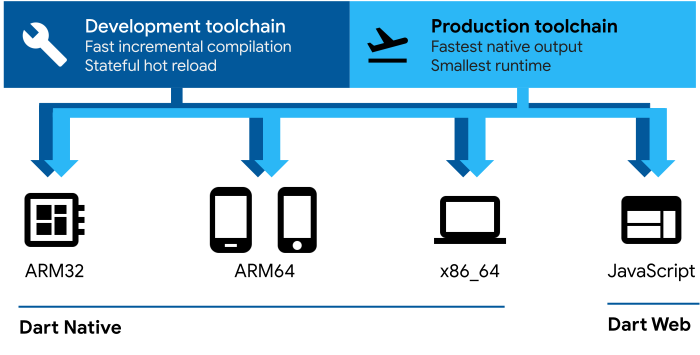
\includegraphics[width=1\textwidth, keepaspectratio=true]{figuras/cap2/2_1_2_dart-platforms.png}
  \centering
  \caption[Plataformas de compilação do Dart]{Plataformas de compilação do Dart \protect\cite{dart-platforms}}
  % \font{Site oficial da linguagem Dart}
  \label{fig:dart_plataforms}
\end{figure}
% \FloatBarrier

Outras características do \textit{Dart} levaram ao seu uso no \textit{Flutter}:

\begin{itemize}
  \item \textbf{ausência de troca de contexto} com a plataforma: como o código compilado é nativo e não possui análises ou novas compilações \textit{JIT}, não há a necessidade de troca de contexto entre a plataforma e a linguagem, o que torna a execução mais rápida;
  % ref: https://hackernoon.com/why-flutter-uses-dart-dd635a054ebf 05/11/2022
  \item \textbf{\textit{single-threaded}}: a preemptividade, isto é, o procedimento de interromper uma tarefa para a execução de outra \textit{thread}, utilizadas em linguagens como \textit{Java} ou \textit{Kotlin} não existe, pois o \textit{Dart} é \textit{single-threaded}, ou seja, não há compartilhamento de memória, nem a necessidade de gerenciamento de estado entre as \textit{threads}, o que evita a possibilidade de erros como condições de corrida ou \textit{deadlock}s;
  \item Uso de \textbf{\textit{isolates}}: todo o código em \textit{Dart} roda dentro de \textit{isolates}, o qual possui um uma única \textit{thread} e se comunica com outros \textit{isolates} por meio de mensagens. Mesmo ações assíncronas são gerenciadas com o uso de classes como \textit{Future} e \textit{Stream} ou com o uso de \textit{async/await}. Dessa forma, o \textit{Dart} é capaz de executar código assíncrono sem a necessidade de novas \textit{threads}. Em última instância, é possível criar um \textit{background isolate}, que será responsável por realizar algum tipo de tarefa em segundo plano, como por exemplo, a leitura ou escrita de um arquivo e devolver seu resultado ao \textit{main isolate} me forma de mensagem quando finalizado.
  % ref: https://dart.dev/guides/language/language-tour#isolates 05/11/2022
% ref: https://dart.dev/guides/language/concurrency#how-isolates-work 05/11/2022
  \item Esquema de \textbf{garbage collection} (GC): a linguagem \textit{Dart} utiliza um avançado esquema de coleta de lixo geracional e que se divide em duas fases. Esse algoritmo favorece a rápida criação e destruição de objetos, o que é comum em aplicações feitas com Flutter, que possui muitos objetos sendo alocados e desalocados, como por exemplo, os \textit{Stateless Widgets}.
  % ref: https://hackernoon.com/why-flutter-uses-dart-dd635a054ebf#:~:text=Allocation%20and%20garbage%20collection 05/11/2022
  % ref: https://medium.com/flutter/flutter-dont-fear-the-garbage-collector-d69b3ff1ca30
\end{itemize}



\section[\textit{Flutter}]{Flutter}
Busca-se apresentar, nesta seção, uma visão em alto nível do que é o \textit{framework Flutter}, sua arquitetura, as principais características da tecnologia e suas diferenças para as demais tecnologias no mercado.

O \textit{Flutter}, criado pela \textit{Google}, é desenvolvido em código aberto e visa possibilitar o desenvolvimento de aplicações \textit{Android}, \textit{Web}, \textit{Desktop} e de \textit{software} embarcado a partir de uma única base de código, compiladas nativamente. A aplicação é mantida não só pela empresa que a criou, mas também recebe novas atualizações e incorporações advindas da comunidade.
% ref: https://docs.flutter.dev/resources/faq#what-is-flutter 30/10/2022


\subsection{Arquitetura do \textit{framework}}
A fazer.
% [A fazer] Falar sobre o hot reload e relacionar com o JIT do Dart VM (https://hackernoon.com/why-flutter-uses-dart-dd635a054ebf#:~:text=a%20game%20changer%E2%80%A6-,Stateful%20hot%C2%A0reload,-One%20of%20the e )
% [A revisar] O \textit{framework} é composto por três camadas principais: \textit{widgets}, \textit{rendering} e \textit{gestures}. A camada de \textit{widgets} é responsável por definir os elementos visuais da aplicação, enquanto a camada de \textit{rendering} é responsável por desenhar os elementos na tela. A camada de \textit{gestures} é responsável por capturar os eventos de interação do usuário com a aplicação, como toques na tela, movimentos do mouse, etc.
% ref: https://flutter.dev/docs/resources/architectural-overview 01/11/2022

\subsection{\textit{Widgets}}
O \textit{framework} recebe inspiração do React e, dessa forma, utiliza-se de \textit{widgets} (\ref{fig:nurse-widget-tree}) para compor os elementos visuais das aplicações, assim como os estados dos mesmos. % ref: https://docs.flutter.dev/development/ui/widgets-intro 01/11/2022
Estes \textit{widgets} devem ser responsáveis por gerir, com boa performance, a renderização dos elementos na tela, suas animações e também controlar as interações do usuário com a aplicação.
% ref.: Wenhao Wu: React Native vs Flutter, cross-platform mobile application frameworks: 2.2.3 Widget: Widgets do not only control and affect how the views behave, but also handle and respond to the user’s action. Thus, it is crucial that Widgets need to perform fast, including rendering and animating. 01/11/2022

\begin{figure}[ht!]
    	
  \centering
          \subfloat[Representação da árvore de \textit{widget}s]{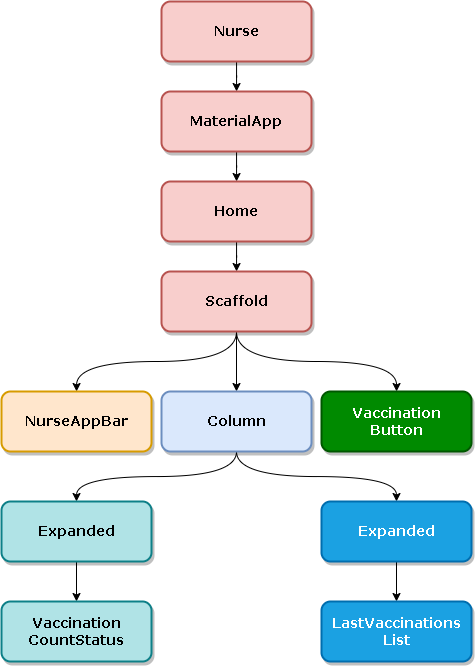
\includegraphics[width=0.45\columnwidth]{figuras/cap2/2_2_2_nurse-widget-tree.png}}
            \qquad
            \subfloat[Árvore apresentada pelo \textit{Flutter DevTools}]{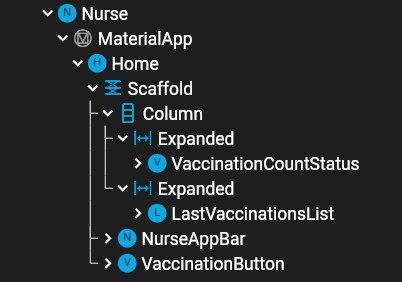
\includegraphics[width=0.45\columnwidth]{figuras/cap2/2_2_2_nurse-widget-tree-flutter-tool.png}}
    \caption[Estrutura simplificada de \textit{widgets} da aplicação \textit{Nurse}]{Estrutura simplificada de \textit{widgets} da aplicação \textit{Nurse}}
  % \fonte{Inserir autor aqui}
  
  \label{fig:nurse-widget-tree}
\end{figure}
% \FloatBarrier
  
Além disso, os \textit{Widgets} devem ser customizáveis e extensíveis, de forma que possam ser flexíveis em relação às suas propriedades e reuso. O Flutter possibilita isso ao trazer a responsabilidade de criação e renderização dos \textit{Widgets} da plataforma à qual está rodando para própria aplicação. Posteriormente, na seção \ref{cap2:Subsec:Diferencas_tecnologias}, será apresentada uma breve explicação da diferença entre o tratamento de \textit{Widgets} feito pelo Flutter e por outras tecnologias, como o \textit{React Native}, \textit{WebViews} e aplicações escritas em Android ou iOS.
 % ref: https://hackernoon.com/whats-revolutionary-about-flutter-946915b09514


A seguir, serão apresentados os dois principais tipos de \textit{widgets} utilizados no desenvolvimento da aplicação, suas principais características e diferenças. São eles: \textit{Stateless Widgets} e \textit{Stateful Widgets}, que diferem entre si, essencialmente, pelo gerenciamento ou não de seu estado interno. % ref: https://docs.flutter.dev/development/ui/widgets-intro 01/11/2022

\subsubsection{Stateless Widgets}
Os \textit{stateless widgets} são \textit{widgets} que não possuem mudança estado, ou seja, não possuem propriedades que podem ser alteradas ao longo do tempo, como por exemplo, quando há uma animação ou um campo de texto ao qual um usuário possa interagir e, assim, só dependem das configurações definidas pelo próprio objeto e o contexto em que ele está inserido. Esses \textit{widgets} podem ser utilizados para representar elementos estáticos da interface, como textos, imagens, botões etc. A seguir, é apresentado um exemplo de um \textit{stateless widget} que representa um botão.
% https://api.flutter.dev/flutter/widgets/StatelessWidget-class.html 01/11/2022
% ref: https://www.youtube.com/watch?v=wE7khGHVkYY 06/11/2022

\begin{lstlisting}[caption={Exemplo de um \textit{stateless widget} que representa um botão.}, label={lst:stateless_widget}]
  class BotaoPrincipal extends StatelessWidget {
    final String texto;
  
    const BotaoPrincipal(Key? key, this.texto) : super(key: key);
  
    @override
    Widget build(BuildContext context) {
      return TextButton(
        onPressed: () => {print("Clicou no botao principal")},
        child: Text(texto),
      );
    }
  }
\end{lstlisting}

No código \ref{lst:stateless_widget} temos a \textbf{classe BotaoPrincipal} que estende um \textit{StatelessWidget} e possui um atributo \textbf{texto} que é passado como parâmetro para o construtor da classe e não pode ser modificado posteriormente (regra garantida pela palavra chave \textit{final} que antecede o tipo da variável). A classe possui um método \textbf{build} que retorna um \textit{widget} do tipo \textit{TextButton} que recebe como parâmetro uma função anônima que imprime uma mensagem no console e um \textit{widget} do tipo \textit{Text} que recebe como parâmetro o atributo \textbf{texto} da classe. No lugar da função de impressão da mensagem em tela poderia ser passado uma função que redireciona o usuário para outra tela, por exemplo.


% https://flutter.dev/docs/development/ui/widgets-intro#stateless-and-stateful-widgets
\subsubsection{Stateful Widgets}

% [A revisar]
Os \textit{stateful widgets} são \textit{widgets} que possuem mudança de estado, ou seja, possuem propriedades que podem ser alteradas ao longo do tempo, como por exemplo, quando há uma animação ou um campo de texto ao qual um usuário possa interagir e, assim, dependem não só das configurações definidas pelo próprio objeto e o contexto em que ele está inserido, mas também do estado interno do objeto. A seguir, é apresentado um exemplo de um \textit{stateful widget} que representa um campo de texto.
% ref: https://api.flutter.dev/flutter/widgets/StatefulWidget-class.html 07/11/2022

% [A revisar]
\begin{lstlisting}[caption={Exemplo de um \textit{stateful widget} que representa um campo de texto.}, label={lst:stateful_widget}]
  class CampoTexto extends StatefulWidget {
    final String texto;

    const CampoTexto({Key? key, required this.texto}) : super(key: key);

    @override
    State<CampoTexto> createState() => _CampoTextoState();
  }

  class _CampoTextoState extends State<CampoTexto> {
    String texto = "";

    @override
    Widget build(BuildContext context) {
      return TextField(
        onChanged: (value) {
          setState(() {
            texto = value;
          });
          print(texto);
        },
        decoration: InputDecoration(
          labelText: widget.texto,
          hintText: "Digite aqui",
        ),
      );
    }
  }
\end{lstlisting}

O \textit{stateful widget} é dividido em duas classes, ou em dois objetos distintos que se contemplam, como pode ser observado no código \ref{lst:stateful_widget}.
% ref: https://medium.com/flutter-community/widget-state-buildcontext-inheritedwidget-898d671b7956 07/11/2022
A primeira classe, a qual estende de \textit{StatefulWidgets} é imutável e também podem receber variáveis via construtor, mas que são finais, assim como as propriedades das classes do tipo \textit{StatelessWidget}'s. Para que hajam mudanças, um objeto do tipo \textit{State} é adicionado e este será responsável pelas mudanças que poderão ocorrer no ciclo de vida do \textit{StatefulWidget}.

A classe que estende \textit{State} (chamada \textbf{CampoTextoState} no exemplo), criada no momento em que a função \textit{StatefulWidget.createState()} é chamada, representa a informação lida pelo \textit{widget} e que pode ser alterada durante o tempo de vida do mesmo.
% ref: https://api.flutter.dev/flutter/widgets/StatefulWidget-class.html 07/11/2022
Além disso, o estado em si pode ter um ciclo de vida maior que o do seu próprio \textit{widget}, mantendo-se em memória mesmo quando este é reconstruído.
% ref: Sebastian Faust: Using Google´s Flutter Framework for the Development of a Large-Scale Reference Application: 3.4.2 Stateful Widgets 07/11/2022

O ciclo de vida de um \textit{State} engloba as seguintes etapas principais:

\begin{enumerate}
  \item criação, a partir da função \textit{createState} e sua associação a um \textit{BuildContext}, responsável por determinar a posição do \textit{widget} que contém o \textit{State} na árvore de \textit{widgets};
  % ref: https://api.flutter.dev/flutter/widgets/BuildContext-class.html
  \item inicialização, com o uso da função \textit{initState}, que também depende do contexto ao qual o widget está associado ou às suas propriedades;
  \item construção, utilizando-se da função \textit{build}, que pode ser chamada inúmeras vezes ao longo do ciclo de vida do \textit{State}, como por exemplo, quando algum dos seus estados internos é alterado;
  \item destruição, com o uso da função \textit{dispose}, que é chamada quando o \textit{State} é removido da árvore de \textit{widgets}.
  % ref: https://api.flutter.dev/flutter/widgets/State-class.html 07/11/2022
\end{enumerate}

Processos intermediários podem ocorrer e funções como \textit{didChangeDependencies} e \textit{didUpdateWidget} são chamadas. Elas podem ser respectivamente utilizadas quando a inicialização do \textit{State} envolve \textit{InheritedWidget}'s ou quando quer-se responder às mudanças provocadas pelo \textit{State} aos seus \textit{widgets} associados.

No código exemplo \ref{lst:stateful_widget} temos a \textbf{classe CampoTexto} que estende um \textit{StatefulWidget} e possui um atributo \textbf{texto} que é passado como parâmetro para o construtor da classe. A classe possui o método \textbf{createState} que retorna um objeto do tipo \textbf{\_CampoTextoState}, uma classe interna da classe \textbf{CampoTexto}.

% [A revisar]
Essa classe interna também possui um atributo \textbf{texto} que é inicializado com uma string vazia e pode ser modificado. O método \textbf{build} retorna um \textit{widget} do tipo \textit{TextField} que, por sua vez, recebe uma função anônima responsável por alterar o estado interno do objeto que, nesse caso, se trata do atributo \textbf{texto}, que recebe o valor passado como parâmetro. Esse método chama a função \textit{setState} que é responsável por notificar o \textit{framework} que o estado interno do objeto foi alterado e que o \textit{widget} deve ser reconstruído.

Além disso, o \textit{widget} do tipo \textit{TextField} recebe como segundo parâmetro um objeto do tipo \textit{InputDecoration} que define o rótulo do campo com o atributo \textbf{texto} da classe \textbf{CampoTexto} e uma dica do que o usuário pode fazer.

\subsubsection{InheritedWidget}

\textit{InheritedWidget} é um tipo especial de \textit{widget} que permite o envio de informações eficientemente entre os nós da árvore de \textit{widgets} que compõe a aplicação. Isto é, a partir de qualquer \textit{widget} descendente de um \textit{InheritedWidget}, pode-se recuperar dados sobre esse componente pai sem que haja a necessidade de repassar a informação por cada um dos nós que compõem o caminho entre os dois, como é demonstrado da imagem \ref{fig:inherited-widget-diagram}.

\begin{figure}[!ht]
  \centering
  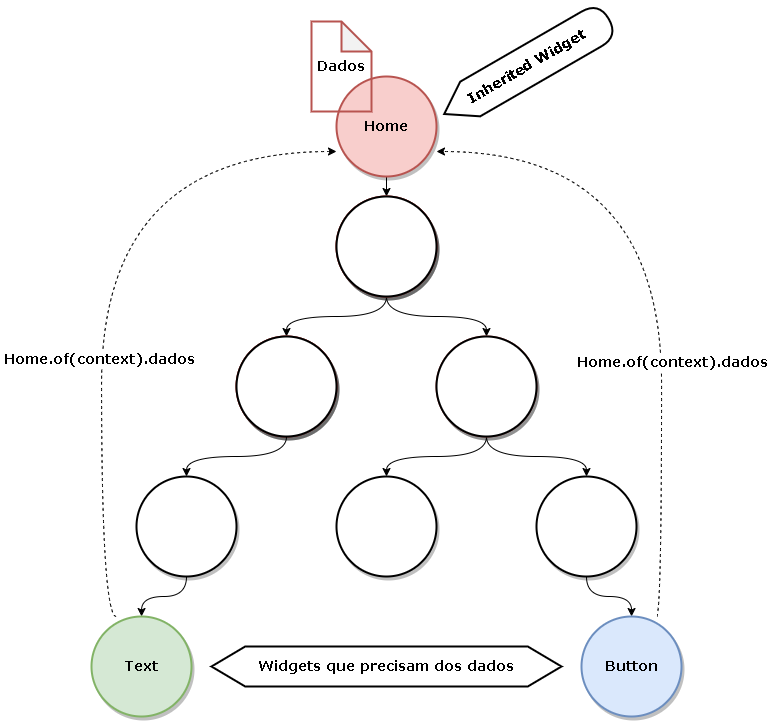
\includegraphics[width=0.8\textwidth]{figuras/cap2/2_2_2_inherited-widget-diagram.png}
  \caption{Exemplo de uma árvore de widgets com InheritedWidget. \protect\cite{Faust2020} \protect\cite{boelens2018}}
  \label{fig:inherited-widget-diagram}
\end{figure}

Neste exemplo, o estado é mantido pelo \textit{widget} nomeado como \textbf{Home} e é acessado pelos \textit{widgets} \textbf{Text} e \textbf{Button} por meio do método estático \textit{Home.of(BuildContext context)} que, por sua vez, busca no contexto dessa sub-árvore, o \textit{widget} mais próximo que seja do exato tipo \textit{Home} e que seja uma extensão concreta da classe InheritedWidget.
% ref: https://api.flutter.dev/flutter/widgets/InheritedWidget-class.html 10/11/2022
% ref: https://api.flutter.dev/flutter/widgets/BuildContext/dependOnInheritedWidgetOfExactType.html 10/11/2022
% \subsection{Principais características}
% A fazer.

\subsection{Diferenças para outras tecnologias}
\label{cap2:Subsec:Diferencas_tecnologias}
A fazer.
 % ref: https://hackernoon.com/whats-revolutionary-about-flutter-946915b09514

\subsection{Gerenciamento de estado}
\label{cap2:Subsec:Gerenciamento_estado}
O gerenciamento de estado no \textit{Flutter} não segue apenas uma arquitetura. Na verdade, o \textit{framework} oferece uma série de opções para que o desenvolvedor possa escolher a que melhor se adapta ao seu projeto \cite{Faust2020}. Algumas das principais opções são: \textit{InheritedWidget}, \textit{Provider}, \textit{MobX} \textit{BLoC} e \textit{Redux}. Cada uma dessas opções possui suas vantagens e desvantagens, sendo que algumas são mais adequadas para projetos pequenos e outras para projetos maiores. Anteriormente, descreveu-se o funcionamento do \textit{InheritedWidget} e, mais a frente, serão apresentadas as principais características sobre o \textit{Provider} e o \textit{MobX}.
% ref: https://docs.flutter.dev/development/data-and-backend/state-mgmt/options 10/11/2022

Antes, porém, é importante destacar que o \textit{Flutter}, diferente de outros \textit{framework}s de desenvolvimento de aplicações \textit{mobile}, como o \textit{Android SDK} e o \textit{iOS UIKit}, não segue uma perspectiva imperativa, onde é possível alterar o estado de um \textit{widget} diretamente. Em vez disso, o \textit{Flutter} segue uma perspectiva declarativa, onde a interface do usuário é alterado através de uma função que retorna um novo \textit{widget}. Isso significa que, ao alterar o estado de um \textit{widget}, o \textit{framework} irá reconstruir esse \textit{widget}, mesmo que isso aconteça a cada novo \textit{frame} da aplicação. O processo pode ser custoso, mas o \textit{Flutter} é rápido o suficiente para isso e existem vantagens associadas, principalmente o benefício de determinar como a interface deve ser construída dado um estado específico e mantê-la assim até que haja a necessidade de uma reconstrução dessa interface.
% ref: https://docs.flutter.dev/development/data-and-backend/state-mgmt/declarative 10/11/2022

\subsection{\textit{Provider}}
\label{cap2:Subsec:Provider}

\textit{Provider} é um \textit{wrapper}, isto é, um encapsulamento que envolve o \textit{InheritedWidget} com o objetivo de simplificar seu uso e, com isso, facilitar o gerenciamento de estados em aplicações \textit{Flutter}.
% ref: https://pub.dev/packages/provider 10/11/2022

Ao utilizar o \textit{Provider}, pode-se encapsular o estado em uma nova classe que herda de \textit{ChangeNotifier} ou se mistura a ela com o uso da palavra reservada \textit{with}, do Dart. Dessa forma, essa classe ganha a capacidade de notificar os \textit{widgets} que se subscrevem a ela quando o estado é alterado. Para isso, basta utilizar o método \textit{notifyListeners()} em métodos que alteram esse estado.
% ref: https://docs.flutter.dev/development/data-and-backend/state-mgmt/simple
% ref: https://www.youtube.com/watch?v=d_m5csmrf7I 10/11/2022

Para fornecer o estado aos widgets que tem interesse nele, utiliza-se o \textit{ChangeNotifierProvider}. Esse \textit{widget} é colocado acima dos widgets que devem receber a instância do \textit{ChangeNotifier}. Por fim, para consumir o estado e responder às suas mudanças, utiliza-se um \textit{widget} chamado \textit{Consumer}, o qual é normalmente colocado ao redor do \textit{widget} que deve ser atualizado quando o estado é alterado. Também pode-se utilizar o método \textit{Provider.of(context)} para obter o estado ou alterá-lo.
% ref: https://docs.flutter.dev/development/ data-and-backend/state-mgmt/simple
% ref: https://www.youtube.com/watch?v=d_m5csmrf7I 10/11/2022

\subsection{\textit{MobX}}
\label{cap2:Subsec:MobX}
% [A revisar]
\textit{MobX} é uma biblioteca para gerenciamento de estado baseado em reatividade \cite{mobx-package}. A reatividade, nesse contexto, é um conceito que permite que o estado de um \textit{widget} mude automaticamente quando uma ação é realizada em outro local, como por exemplo, um outro \textit{widget}. Para isso, utiliza-se a ideia de observabilidade a partir do \textit{widget} que depende do estado a ser observado e, assim que este é alterado, o \textit{widget} é notificado e reconstruído. Esse ciclo pode ser demonstrado na imagem \ref{fig:mobx-cycle}.


\begin{figure}[!ht]
  \centering
  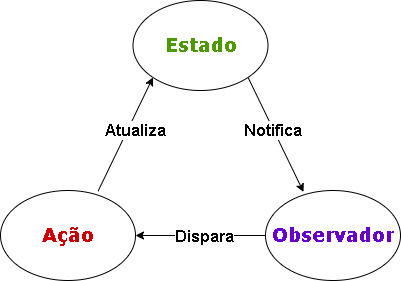
\includegraphics[width=0.6\textwidth]{figuras/cap2/2_2_6_mobx-cycle.png}
  \caption{Ciclo básico do gerenciamento de estado com o MobX \protect\cite{mobx-package} \protect\cite{podila18mobx}}
  \label{fig:mobx-cycle}
\end{figure}


A \textbf{ação} é responsável por gerar mudança no estado da aplicação. Ela pode ser disparada por uma interação do usuário com algum \textit{widget}, como um botão, assim como pode ser resposta a um efeito colateral causado por uma outra ação anterior a esta e que gerou uma mudança de estado anterior, a qual foi consumida por um observador.

O \textbf{observador}, por sua vez, pode ser um \textit{widget}, que apresentará uma mudança visual ao usuário ou uma função responsável por lidar com a mutação desse estado, mas sem que haja, necessariamente, uma reconstrução da interface.

E, por fim, o \textbf{estado} é o valor que será observado e que, quando alterado, notificará os observadores. Esse estado pode ser uma variável, um objeto ou uma lista de objetos, por exemplo.

A notificação realizada pelo estado pode ocasionar efeitos colaterais em outros observadores, que por sua vez, podem disparar novas ações, gerando um ciclo de reatividade. A imagem \ref{fig:mobx-details} apresenta uma representação mais detalhada do ciclo com o \textit{MobX}.

\begin{figure}[!ht]
  \centering
  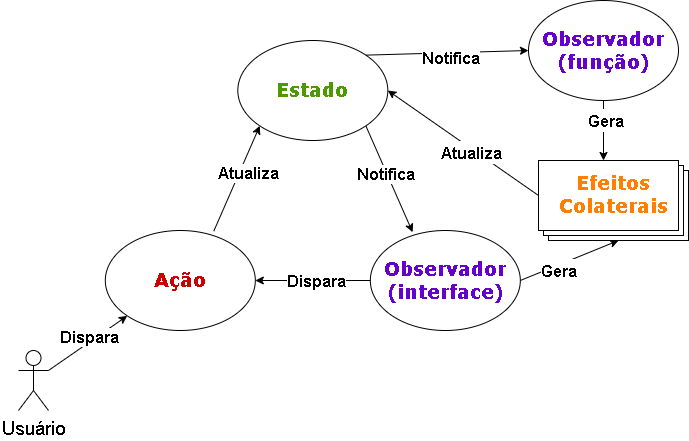
\includegraphics[width=0.9\textwidth]{figuras/cap2/2_2_6_mobx-details.png}
  \caption{Ciclo detalhado do gerenciamento de estado com o MobX \protect\cite{mobx-package} \protect\cite{podila18mobx}}
  \label{fig:mobx-details}
\end{figure}

% [A analisar] [A fazer] Exemplo genérico da implementação do MobX.


% \section{Programação Orientada a Objetos}
% A fazer.

\section{Persistência de Dados}
% [A revisar]
A persistência de dados no contexto do Flutter é o processo de armazenamento em disco das informações relativas à aplicação ou ao seu usuário.
A persistência de dados em um aplicativo móvel permite que o usuário possa acessar as informações mesmo quando não estiver conectado à internet ou mesmo quando o aplicativo estiver fechado. As principais formas de armazenamento de dados em uma aplicação Flutter são: salvamento em \textit{Shared Preferences}, leitura e escrita de arquivos e salvamento em banco de dados \textit{SQLite} \cite{persistence}.
% ref: https://docs.flutter.dev/cookbook#persistence 12/11/2022

A forma como as informações são salvas dependem da quantidade, complexidade e finalidade delas. Para pequenos conjunto de dados, o salvamento em chave-valor, utilizando o \textit{Shared Preferences}, é uma boa opção \cite{shared_preferences}. Já para arquivos de texto, como por exemplo, um arquivo \textit{JSON}, o salvamento em disco é uma boa opção, pois permite a leitura e escrita de dados de forma mais abrangente em relação ao tipo de arquivo salvo e sua utilidade posterior \cite{reading_writing_files}. Por fim, para grandes conjuntos de dados, como por exemplo, uma lista de contatos, o \textit{SQLite} é preferível, pois ele é uma biblioteca que implementa o mecanismo de um banco de dados relacional \cite{sqlite-org} que permite a criação de tabelas e a manipulação de dados de forma simples e rápida \cite{sqlite-flutter} \cite{sqlite_features}.

No contexto da aplicação, a quantidade de dados pode ser consideravelmente grande e estão bastante relacionados entre si, como descrito na \ref{Sec:DiagramaClasses}. Por conta disso, a estratégia utilizada é a de salvar os dados em banco relacional, utilizando o \textit{SQLite}.

\subsection{\textit{Banco de Dados SQLite}}
Um banco de dados pode ser entendido como um conjunto organizado e integrado de dados ou informações que atendem a um conjunto de usuários \cite{heuser09banco} \cite{oracle}. Em geral, os bancos de dados tem o objetivo de armazenar dados de vários sistemas e/ou usuários diferentes e, por conta disso, utilizam-se de sistemas de gerenciamento de banco de dados (SGBD) modularizados \cite{heuser09banco} que, em alguns casos, exigem um servidor a parte para realizar os processos que recebem em uma arquitetura conhecida como cliente/servidor \cite{sqlitetutorial_net}.

Para esse tipo de banco de dados, o foco está mais atrelado à escalabilidade e concorrência de dados, visto que inúmeros novos sistemas podem ser acoplados ao banco de dados pré-existente. No caso do \textit{SQLite}, o foco está mais voltado para a economia, eficiência e simplicidade, ao passo em que ele atenderá a um único sistema ou aplicação que, nesse caso, se trata do dispositivo móvel e dos poucos usuários (em geral, apenas um), que o utilizarão \cite{sqlite_use}.

\subsection{Modelagem do banco de dados}
\label{Sec:ModelagemBD}

A modelagem dos dados que serão salvos em um banco fornece uma representação abstrata da estrutura das informações que estarão contidas ali. Essa modelagem normalmente segue dois níveis de abstração diferentes que são criados de acordo com a finalidade e com o momento de desenvolvimento do projeto. O \textbf{modelo conceitual} normalmente possui informações menos detalhadas, mas que passam uma ideia geral da estrutura que será criada no banco de dados e os tipos de informação que estarão presente. Posteriormente, cria-se um \textbf{modelo lógico}, o qual já depende do SGBD utilizado e possui mais detalhes sobre os tipos de informações que possui e a forma como elas serão gravadas. \cite{heuser09banco}.

A seguir, na figura \ref{fig:diagrama_er}, é apresentada um exemplo de modelagem conceitual do banco de dados, utilizando-se uma parte simplificada da aplicação e, na figura \ref{fig:diagrama_logico}, a modelagem lógica para a mesma parte da aplicação.

\begin{figure}[!ht]
    \centering
    
\includegraphics[width=0.8\textwidth]{figuras/cap2/2_3_2_diagrama-er.png}
    \caption{Modelagem conceitual de parte do banco de dados}
    \label{fig:diagrama_er}
\end{figure}

\begin{figure}[!ht]
    \centering
    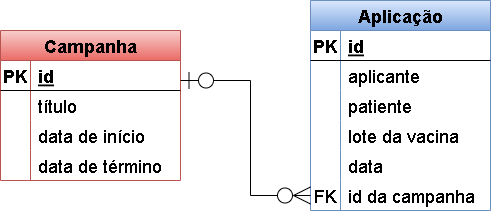
\includegraphics[width=0.8\textwidth]{figuras/cap2/2_3_2_diagrama-logico.png}
    \caption{Modelagem lógico de parte do banco de dados}
    \label{fig:diagrama_logico}
\end{figure}

Observa-se que a notação utilizada no relacionamento entre as entidades 'Campanha' e 'Aplicação', para ambas as modelagens, segue o padrão conhecido como notação Engenharia de Informações. Nesse tipo de notação, a relação é demonstrada por uma linha e a cardinalidade é representada pelos símbolos nas extremidades dessa linha, ligados à entidade. Ademais, a denominação do relacionamento é dado pelas frases verbais que estão presentes na relação  \cite{heuser09banco}. No caso do relacionamento 'Campanha' e 'Aplicação', ele é representado por 'realiza' e 'é realizada em'.

% ref: [cap 1]
% ref: [cap 5: intro] do livro do heuser


%ref: Projeto de Banco de Dados - C. A. Heuser: Capítulo 1: Seção 1.1.1:  A solução para evitar a redundância não controlada de informações é o compartilhamento de dados. Nesta forma de processamento, cada informação é armazenada uma única vez, sendo acessada pelos vários sistemas que dela necessitam (Figura 1.2). \textit{Ao conjunto de arquivos integrados que atendem a um conjunto de sistemas dá-se o nome de banco de dados (BD)}.

% \section{Arquitetura de Sistemas}
% A fazer.

% \section{Princípios SOLID}

% \subsection{Single Responsibility Principle}
% A fazer.

% \subsection{Open/Closed Principle}
% A fazer.

% \subsection{Liskov Substitution Principle}
% A fazer.

% \subsection{Interface Segregation Principle}
% A fazer.  

% \subsection{Dependency Inversion Principle}
% A fazer.



% % Cap. 3 - Trabalhos Relacionados
% %%
%% Capítulo 2: Expressões matemáticas
%%

\mychapter{Trabalhos relacionados}
\label{Cap:TrabalhosRelacionados}

% Escrever sobre os trabalhos relacionados ao projeto. Dois exemplos dele estão na pasta de arquivos que eu baixei, sobre o desenvolvimento de aplicações em larga escala.

% \cite{art-solimaes03}, \cite{col-pinto00}, ..

% Cap. 4 - Problema
% %%
%% Capítulo 4: Problema
%%

\mychapter{Problema}
\label{Cap:Problema}


% Cap. 4 - Nurse: uma aplicação para produtividade em vacinações
%%
%% Capítulo 4: Nurse: uma aplicação para produtividade em vacinações
%%

\mychapter{Nurse: uma aplicação para produtividade em vacinações}
\label{Cap:Implementacao}
Nessa seção, os requisitos e casos de usos da aplicação serão descritos. Além disso, será apresentada a arquitetura escolhida para a aplicação, tanto no sentido das camadas hierárquicas de responsabilidade \cite{Faust2020}, quanto na divisão de pastas e subpastas dos arquivos que compõem o código em módulos e, por fim, as telas do aplicativo e os pacotes utilizados para o desenvolvimento das funcionalidades serão mostrados.

O projeto foi desenvolvido utilizando a linguagem de programação \textit{Dart}, com o \textit{framework Flutter}. O seu repositório pode ser encontrado no \textit{GitHub}, em \url{https://github.com/Dojak220/nurse}. A documentação, que inclui a versão dessa monografia em formato \textit{pdf} e o seu respectivo projeto em \LaTeX também pode ser encontrada no \textit{Github}, em \url{https://github.com/Dojak220/nurse-docs}.
% [A fazer] Criar um GitHub Pages \url{https://dojak220.github.io/nurse/}.

\section{Requisitos do Sistema}
\label{cap4:Sec:Requisitos}

Os requisitos da aplicação foram definidos de acordo com a análise feita a partir do problema identificado e com os objetivos descritos nas seções \ref{cap1:Sec:Problematica} e \ref{cap1:Sec:Objetivos}, respectivamente. Em suma, eles foram definidos com o intuito de suprir as necessidade de seus usuários com base naquilo que quer-se resolver. Esses requisitos, por sua vez, podem ser divididos em três tipos: funcionais, não funcionais e de domínio. Certos requisitos podem não estar claramente definidos como uma das três opções acima e, em alguns casos, um dado requisito pode se subdividir em mais requisitos menores e de tipos diferentes daquele que o originou \cite{sommerville2007engineering}. 

\subsection{Requisitos Funcionais}
\label{cap4:Subsec:RequisitosFuncionais}
Os requisitos funcionais (RF) são aqueles que descrevem as funcionalidades que o sistema deve possuir para atender às necessidades do usuário \cite{sommerville2007engineering}. A seguir (tabela \ref{tab:rf}), são apresentados os requisitos funcionais do sistema e os detalhes para alguns deles podem ser encontrados no apêndice \ref{apendice:requisitos_funcionais_detalhados}.

\begin{table}[ht!]
  \centering
  {\rowcolors{0}{white}{green!20}
  \begin{tabularx}{\textwidth}{
    | >{\centering\arraybackslash}m{0.10\textwidth} 
    | >{\centering\arraybackslash}X 
    | >{\raggedright\arraybackslash}X | }
    \hline
    \rowcolor{green!100}
    \textbf{Código} & \textbf{Requisito} & \textbf{Descrição} \\ \hline \hline
    RF01  &  Cadastrar entidades              & Permitir que o usuário cadastre novas entidades (sub-requisitos na tabela \ref{tab:rf01_detalhe}) \\ \hline
    RF02  &  Visualizar entidades cadastradas & Permitir que o usuário visualize as entidades cadastradas e seus detalhes (sub-requisitos na tabela \ref{tab:rf02_detalhe}) \\ \hline
    RF03  &  Editar entidades                 & Permitir que o usuário edite entidades já cadastradas seguindo fluxo análogo ao cadastro de nova entidade, porém, com campos pré-preenchidos \\ \hline
    RF04  &  Gerar tabela de vacinações       & Permitir que o usuário gere uma tabela de vacinações para exportação (sub-requisitos na tabela \ref{tab:rf04_detalhe}) \\ \hline
  \end{tabularx}}
\caption{Requisitos funcionais da aplicação Nurse}
\label{tab:rf}
\end{table}

\subsection{Requisitos Não Funcionais}
\label{cap4:Subsec:RequisitosNaoFuncionais}

Os requisitos não funcionais (RNF) são aqueles que descrevem as características do sistema que não são diretamente implementadas como uma funcionalidade específica na aplicação, mas que são importantes para o seu funcionamento, como o nível de confiabilidade da aplicação, performance e segurança. Além disso, são esses requisitos que apresentam as restrições inerentes à aplicação \cite{sommerville2007engineering}. A seguir (tabela \ref{tab:rnf}), são apresentados os requisitos não funcionais do sistema.

\begin{table}[ht!]
  \centering
  {\rowcolors{0}{white}{green!20}
  \begin{tabularx}{\textwidth}{
    | >{\centering\arraybackslash}m{0.10\textwidth} 
    | >{\centering\arraybackslash}X 
    | >{\raggedright\arraybackslash}X | }
    \hline
    \rowcolor{green!100}
    \textbf{Código} & \textbf{Requisito} & \textbf{Descrição} \\ \hline \hline
    RNF01  &  Correta estrutura dos dados              & Garantir que os dados fornecidos pelo usuário sejam aceitos e salvos apenas se seguirem as especificações e regras relativas a eles (por exemplo, CPF que deve seguir um conjunto de regras para ser considerado válido)   \\ \hline
    RNF02  &  Dados em planilha & Apenas os dados referentes às vacinações devem postos em uma planilha e esta deve seguir o formato apresentado na seção \ref{cap1:SubSec:CenariosVacinacao}) \\ \hline
    RNF03  &  Cadastros não podem ser apagados  & As informações que forem salvas sobre qualquer uma das entidades pelo usuário não devem ser apagadas. Elas podem apenas ser alteradas (funcionalidade RF03) \\ \hline
  \end{tabularx}}
\caption{Requisitos não funcionais da aplicação Nurse}
\label{tab:rnf}
\end{table}
% [A fazer] Mostrar planilha de preenchimento da vacinação e os campos apresentados. Além disso, mostrar a planilha que deve ser exportada na plataforma.

\subsection{Casos de Uso}
\label{cap4:Subsec:CasosDeUso}

Uma das formas de representar um sistema, seu escopo e limites é através da identificação dos seus casos de uso e dos atores que interagem com o sistema \cite{schneider2001applying}. Estes atores podem ser desde pessoas a outras aplicações e os casos de uso descrevem o que os atores querem que o sistema realize. A seguir, na Figura \ref{fig:casos_de_uso}, é apresentado o diagrama dos casos de uso da aplicação Nurse e, logo abaixo, a tabela \ref{tab:actors} com a descrição dos atores envolvidos.

\begin{figure}[!ht]
  \centering
  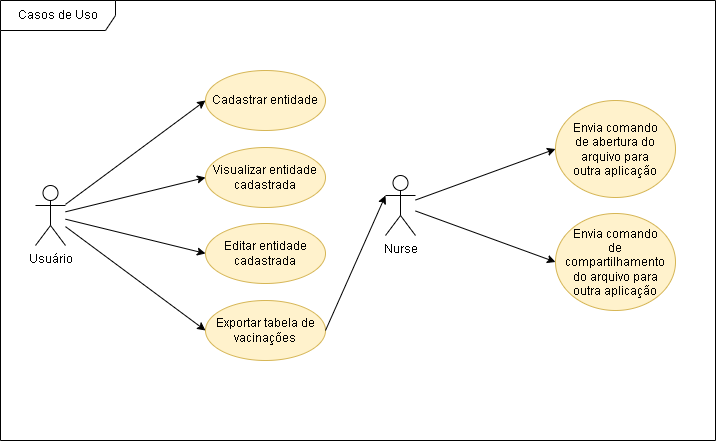
\includegraphics[width=\textwidth]{figuras/cap4/4_1_3_use_cases.png}
  \caption{Diagrama de casos de uso da aplicação Nurse}
  \label{fig:casos_de_uso}
\end{figure}

\begin{table}[ht!]
  \centering
  {\rowcolors{0}{white}{green!20}
  \begin{tabularx}{\textwidth}{
    | >{\centering\arraybackslash}m{0.15\textwidth} 
    | >{\centering\arraybackslash}X |}
    \hline
    \rowcolor{green!100}
    \textbf{Ator} & \textbf{Descrição} \\ \hline \hline
    Usuário & Usuário que utiliza a aplicação Nurse para gerenciar os dados das vacinações realizadas \\ \hline
    Nurse & É a própria aplicação utilizada, mas que também realiza chamada para abertura e/ou compartilhamento de planilhas em outras aplicações \\ \hline
  \end{tabularx}}
\caption{Descrição dos atores envolvidos na aplicação Nurse}
\label{tab:actors}
\end{table}

\section{Arquitetura do Sistema}
\label{cap4:Sec:ArquiteturaSistema}

A definição de uma arquitetura para o desenvolvimento de um projeto é essencial para que o mesmo seja desenvolvido de forma organizada e eficiente, mas também tornar a sua manutenção mais simples. Em outras palavras, o objetivo em definir uma arquitetura é diminuir os recursos humanos e, consequentemente, financeiros necessários durante todo o ciclo de vida de um projeto, desde a sua concepção até a sua manutenção, passando pelo desenvolvimento de suas funcionalidades \cite{martin2019arquitetura}. 

Para se alcançar esse objetivo, pode-se utilizar de técnicas, como as supracitadas divisão em camadas de responsabilidade e a modularização, entre outras. Além disso, é importante construir um modelo do domínio-problema da aplicação para que as complexidades inerentes a ele sejam melhor controladas \cite{evans2017domain}. O domínio, ou seja, a área na qual a aplicação Nurse está inserida e qual problema quer-se resolver, engloba do todo o conjunto de ações necessárias para realizar uma vacinação, desde o cadastro das entidades envolvidas (paciente, aplicante, vacina etc...) até a posterior exportação dos dados coletados. O modelo criado para o banco de dados é usado para modelar as entidades envolvidas e a relação entre elas, já as classes desenvolvidas para criar os arquivos a serem exportados é um exemplo da implementação no código das ações necessárias dentro desse domínio-problema.

\subsection{Camadas de Responsabilidade}
\label{cap4:SubSec:CamadasResponsabilidade}
A divisão em camadas hierárquicas de responsabilidade tem como objetivo dividir o projeto em partes menores, cada uma com uma responsabilidade específica e de forma a torná-las o mais independente possível entre elas \cite{Faust2020} e, dessa forma, diminuir o acoplamento e aumentar a coesão das classes. Um exemplo desse tipo de arquitetura é o sistema MVC (Model-View-Controller), que divide o projeto em três camadas: a \textbf{camada de modelo}, que contém as classes que representam as entidades do domínio-problema e gerencia os dados associados a elas; a \textbf{camada de visualização}, que contém as classes que representam as telas da aplicação e gerenciam as suas mudanças textuais e gráficas; e a \textbf{camada de controle}, que contém as classes que intermedeiam as outras duas camadas ao interpretar as ações do usuário e enviar comandos às classes do modelo e/ou da visualização para realizar quaisquer mudanças necessárias \cite{burbeck1987mvc}.

Essa divisão pode ser realizada em \textit{n} camadas. No caso da aplicação Nurse, dividiu-se o projeto em cinco, como mostrado na figura \ref{fig:4_1_1_camadas_nurse}.

\begin{figure}[!ht]
  \centering
  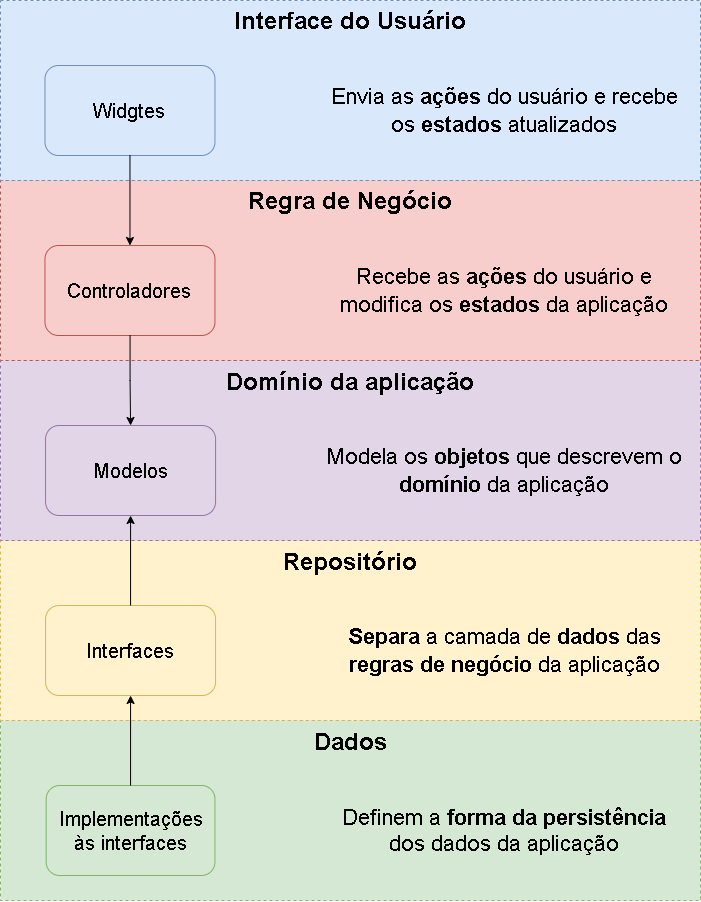
\includegraphics[width=0.6\textwidth]{figuras/cap4/4_1_1_camadas_nurse.png}
  \caption{Camadas da aplicação \textbf{Nurse} e suas dependências}
  \label{fig:4_1_1_camadas_nurse}
\end{figure}

\subsubsection{Interface do Usuário}
\label{cap4:SubSubSec:UI}
Engloba todos os elementos (\textit{widgets}) visuais e de interação com o usuários, como campos de texto ou botões, cores, imagens, ícones, etc... Essa camada é responsável por receber os comandos do usuário e enviar comandos para as outras camadas, como a camada de controle, para que as ações necessárias sejam realizadas. Além disso, é responsável por gerenciar as mudanças de estado da interface, como a mudança de cor de um botão ao ser clicado, por exemplo. As telas apresentadas na seção seguinte (\ref{cap4:Sec:Telas}) mostram esses elementos com mais detalhes.

\subsubsection{Camada de Regra de Negócio}
\label{cap4:SubSubSec:RegraNegocio}
% [A revisar]
A camada de controle recebe as ações tomadas pelo usuário na camada de interface e toma decisões a partir delas. Essas decisões são tomadas com base nas regras de negócio da aplicação (daí o nome da camada). Essas regras são implementadas em classes que fazem parte dessa camada, aqui nomeadas como \textbf{Controladores}.

Por exemplo, a classe \textit{AddPatientFormController} é responsável por gerenciar as ações relacionadas às páginas de inserção de um novo paciente ou de edição de outro já cadastrado. Durante o preenchimento dos dados nos campos de texto e de seleção em lista suspensa, essa classe salva os dados em um objeto que representa um paciente e, ao tentar salvar, verifica-se a validade dos dados inseridos pelo usuário e se esse cadastro já não havia sido realizado. Caso algum desses requisitos não seja atendido, um estado de erro é enviado à camada anterior para que esta apresente uma mensagem ao usuário, caso contrário, o objeto (um novo paciente, nesse exemplo) é enviado à camada responsável por salvá-lo no banco de dados e o usuário é redirecionado para a página de listagem de pacientes, onde poderá ver o novo item adicionado.

Vale ressaltar que essa validação, assim como o salvamento dos dados, não é responsabilidade dos controladores, então essas ações são delegadas a outras classes e/ou camadas e apenas os resultados que interessam aos controladores são retornados. A seguir, no trecho de código \ref{lst:patient_form_controller} são apresentados alguns detalhes da classe \textit{AddPatientFormController}, ressaltando o uso do \textit{MobX} e os métodos que conectam as camadas adjacentes à da regra de negócio.

\begin{lstlisting}[caption={Trechos da classe \textit{PatientFormController}}, label={lst:patient_form_controller}]
  class AddPatientFormController = _AddPatientFormControllerBase
      with _$AddPatientFormController;

  abstract class _AddPatientFormControllerBase extends AddFormController
      with Store {
    // ...

    @observable
    ObservableList<Locality> localities =
      ObservableList.of(List<Locality>.empty(growable: true));

    @observable
    ObservableList<PriorityCategory> categories =
      ObservableList.of(List<PriorityCategory>.empty(growable: true));
      
    @observable
    PatientStore patientStore = PatientStore();

    final Patient? initialPatientInfo;

    _AddPatientFormControllerBase(this.initialPatientInfo) {
      if (initialPatientInfo != null) {
        patientStore.setInfo(initialPatientInfo!);
      }
  
      getLocalities();
      getPriorityCategories();
    }

    @action
    Future<List<Locality>> getLocalities() async {
      final localities = await _localityRepository.getLocalities();

      this.localities
        ..clear()
        ..addAll(await _localityRepository.getLocalities());

      return localities;
    }

    @action
    Future<List<PriorityCategory>> getPriorityCategories() async {
      // ...
    }

    @override
    Future<bool> saveInfo() async {
      if (submitForm(formKey)) {
        final PatientStore p = patientStore;
        
        // ...

      } else {
        return false;
      }
    }

    @override
    Future<bool> updateInfo() async {
      if (initialPatientInfo == null) return false;

      if (submitForm(formKey)) {
        final PatientStore p = patientStore;
        
        // ...

      } else {
        return false;
      }
    }

    // ...
  }
\end{lstlisting}

Inicialmente, na declaração da classe, utilizou-se o padrão sugerido na própria documentação do \textit{mobx} no Flutter para geração automática de código por meio do pacote de desenvolvimento \textit{mobx\_codegen} \cite{mobx_core_concepts}. Essa geração torna mais simples a utilização dos recursos do \textit{MobX}, como os \textit{\textbf{Observables}} e \textit{\textbf{Actions}} e, por isso, foi utilizada. Adiciona-se à declaração, uma extensão à classe abstrata \textit{AddFormController}, responsável por definir métodos comuns a todas as classes de controle de formulários de inserção de dados como, por exemplo, os métodos \textit{saveInfo} e \textit{updateInfo}.

Em seguida, podemos observar três propriedades observáveis, sendo duas listas e um objeto do tipo \textbf{\textit{PatientStore}} que, por sua vez, também possui propriedades observáveis internamente. É nessa última que estão os valores sobre o paciente, enviados pelo usuário na interface, como mostra o trecho de código \ref{lst:patient_store}. Nesse exemplo são mostradas algumas propriedades e métodos responsável por atualizá-las.

\begin{lstlisting}[caption={Trechos da classe \textit{PatientStore}}, label={lst:patient_store}]
  class PatientStore = _PatientStoreBase with _$PatientStore;

  abstract class _PatientStoreBase with Store {
    @observable
    Locality? selectedLocality;

    @observable
    String? cns;
  
    @observable
    String? name;

    ...outras propriedades

    @action
    void setLocality(Locality? value) => selectedLocality = value;
  
    @action
    void setCns(String value) => cns = value;
  
    @action
    void setName(String value) => name = value;
  
    // ...outros metodos
  
    @action
    void setInfo(Patient patient) {
      selectedLocality = patient.person.locality;
      selectedBirthDate = patient.person.birthDate;
      cns = patient.cns;
      name = patient.person.name;

      // ...
    }
  
    @action
    void clearAllInfo() {
      selectedLocality = null;
      selectedBirthDate = null;
      cns = null;
      name = null;

      // ...
    }
  }
  
\end{lstlisting}

De volta à listagem \ref{lst:patient_form_controller}, logo após as propriedades observáveis, temos os métodos \textbf{\textit{getLocalities}} e \textit{\textbf{getPriorityCategories}}, que agem como ações (marcadas com o \textit{@action}) e são responsáveis por buscar as informações necessárias para preencher as listas usadas para seleção de localidade e categoria de prioridade, respectivamente. Esses métodos são chamados no construtor da classe (simplificado nesse trecho de código), que recebe como parâmetro um objeto do tipo \textit{Patient}, que é utilizado para preencher os campos do formulário quando o usuário deseja editar um paciente já existente. Essa classe também possui os métodos \textit{saveInfo} e \textit{updateInfo} que são responsáveis por salvar e atualizar os dados do paciente no banco de dados, respectivamente.

\subsubsection{Domínio da Aplicação}
\label{cap4:SubSubSec:Dominio}
Nessa camada estão as classes que representam as entidades do domínio-problema da aplicação. Observa-se que essa camada não depende de nenhuma outra e pode ser considerada aquela que vai dirigir as implementações das demais \cite{evans2017domain}. Essas classes são definidas com base no mesmo modelo descrito, com mais detalhes, na seção \ref{cap4:SubSec:DiagramaClasses}. No trecho de código \ref{lst:vaccine_model} a seguir, é possível ver como a classe \textit{Vaccine}, que modela uma vacina presente no domínio do problema, é implementada.

\begin{lstlisting}[caption={Trecho da implementação da classe \textbf{Vaccine}}, label={lst:vaccine_model}]
  class Vaccine implements GenericModel {
    @override
    final int? id;
    final String sipniCode;
    final String name;
    final String laboratory;

    Vaccine({
      this.id,
      required String sipniCode,
      required String name,
      required String laboratory,
    })  : sipniCode = sipniCode.trim(),
          name = name.trim(),
          laboratory = laboratory.trim() {
      _validateVaccine();
    }

    void _validateVaccine() {
      if (id != null) Validator.validate(ValidatorType.id, id!);
      Validator.validateAll([
        ValidationPair(ValidatorType.numericalString, sipniCode),
        ValidationPair(ValidatorType.name, name),
        ValidationPair(ValidatorType.name, laboratory),
      ]);
    }
    ...
  }
\end{lstlisting}

A partir dessa classe, podemos verificar aquilo que compõe essa camada. A classe em si representa o que seria a vacina aplicada pelo profissional da saúde dentro de um processo de vacinação a um paciente e, portanto, é uma entidade do domínio-problema. Interno a essa classe estão os atributos que representam as informações que a vacina possui, como o seu nome, seu código SIPNI e o laboratório que a produziu. Além disso, é possível ver que a classe implementa a interface \textit{GenericModel}, que é uma interface que define os atributos e métodos que devem ser implementados por todas as classes que representam entidades do domínio-problema. Essa interface é definida no arquivo \textit{generic\_model.dart} e pode ser vista no trecho de código \ref{lst:generic_model} a seguir.

\begin{lstlisting}[caption={Interface \textbf{GenericModel}}, label={lst:generic_model}]
  abstract class GenericModel {
    final int? id;
  
    GenericModel(this.id);
  
    Map<String, dynamic> toMap();
  }
\end{lstlisting}

A classe \textit{Vaccine} também implementa os métodos \textit{fromMap} e \textit{toMap}, que são responsáveis por converter um objeto dessa classe em um \textit{Map} e vice-versa. Esses métodos são utilizados pelos repositórios para salvar e recuperar os dados.

Há, também, um processo de validação realizado pelo \textbf{\textit{Validator}}. Essa classe de suporte transita entre as camadas de domínio e de regra de negócio, pois ela é utilizada pelos \textit{models} para garantir que as informações que estão tentando ser cadastradas são válidas de acordo com as regras que definem o domínio-problema. Caso haja algum erro, essa informação é devolvida enviada para a camada de regra de negócio.

\subsubsection{Camada de Repositório}
\label{cap4:SubSubSec:Repositorio}

A camada de repositório separa a camada de dados da camada da regra de negócio \cite{Faust2020} \cite{andrea_repositories}. Ela é responsável por abstrair a forma como os dados são armazenados, permitindo que a aplicação seja portada para diferentes bancos de dados ou para API's sem que seja necessário alterar a regra de negócio. Essa camada é composta por classes abstratas que definem uma interface com os métodos a serem implementados pelas classes que utilizam-se dessa interface. A seguir, no trecho de código \ref{lst:campaign_repository}, é apresentada a interface \textbf{CampaignRepository} e sua implementação para uso de banco de dados, \textbf{DatabaseCampaignRepository}, pode ser vista no trecho de código \ref{lst:database_campaign_repository}, na seção \ref{cap4:SubSubSec:Dados}.

\begin{lstlisting}[caption={Interface \textbf{CampaignRepository}}, label={lst:campaign_repository}]
  abstract class CampaignRepository {
    Future<int> createCampaign(Campaign campaign);
    Future<int> deleteCampaign(int id);
    Future<Campaign> getCampaignById(int id);
    Future<Campaign> getCampaignByTitle(String title);
    Future<List<Campaign>> getCampaigns();
    Future<int> updateCampaign(Campaign campaign);
  }
\end{lstlisting}

Pode-se observar que a classe \textbf{CampaignRepository} define seis funções relacionadas à criação, atualização, busca e remoção de campanhas de vacinação. Contudo, ela não determina como essas funções devem ser implementadas, apenas que as sejam. Dentro da camada de regra de negócio, a dependência, as classes recebem como dependência um objeto do tipo \textbf{CampaignRepository} e, dessa forma, não precisam se preocupar com a forma como os dados serão armazenados, mas apenas garantir que a chamada às funções de armazenamento sigam a assinatura da interface definida. No trecho de código a seguir (\ref{lst:campaign_repository_usage}) é apresentado um exemplo de de uso.

\begin{lstlisting}[caption={Exemplo de uso da interface \textbf{CampaignRepository}}, label={lst:campaign_repository_usage}]
  class AddCampaignFormController extends AddFormController {
    final CampaignRepository _repository;
    
    ...
  
    AddCampaignFormController(
        [CampaignRepository? campaignRepository])
        : _repository = campaignRepository ?? DatabaseCampaignRepository() {...}
    }

    ...
  }
\end{lstlisting}

A classe de controle da adição de novas campanhas de vacinação recebe o repositório \textbf{CampaignRepository} como parâmetro no construtor. Dessa forma, ao criar-se uma instância desse controlador, é possível passar um repositório diferente, como um repositório que armazena os dados em um banco de dados relacional ou outro que utiliza um banco de dados não relacional. Como, nesse projeto, utiliza-se apenas uma forma de armazenamento, definiu-se como repositório padrão o \textbf{DatabaseCampaignRepository}, contudo, ainda é possível passar outros tipos de repositório como parâmetro sem a necessidade de mudar nenhuma linha de código dentro do controlador.

\subsubsection{Camada de Dados}
\label{cap4:SubSubSec:Dados}

É nessa camada que serão realizadas as implementações dos repositórios definidos na camada de repositório. Nesse projeto, foi utilizado o banco de dados SQLite para armazenar os dados, como será melhor explicado nas seções \ref{cap4:Subsec:sqflite-sqlcipher-package} e \ref{cap4:Sec:PersistenciaDados}.

No trecho de código abaixo (\ref{lst:database_campaign_repository}) é apresentada a implementação do repositório \textbf{DatabaseCampaignRepository}. Pode-se observar que a classe implementa a interface \textbf{CampaignRepository} e, portanto, deve implementar todos os métodos definidos nessa interface (apenas dois dos métodos foram apresentados aqui, pois os outros possuem uma estrutura análoga a estes). Além disso, a classe herda de \textbf{DatabaseInterface} que, por sua vez, define métodos de acesso ao banco de dados que serão utilizados por todas as classes concretas de repositórios que realizam esse tipo de armazenamento.

Tanto a classe \textbf{DatabaseInterface} como a classe \textbf{DatabaseManager}, que é utilizada pela primeira, serão melhor descritas na seção \ref{cap4:Sec:UsoBancoDados}.

\begin{lstlisting}[caption={Implementação na classe \textbf{DatabaseCampaignRepository} da interface \textbf{CampaignRepository}}, label={lst:database_campaign_repository}]
  class DatabaseCampaignRepository extends DatabaseInterface
      implements CampaignRepository {
    // ignore: constant_identifier_names
    static const String TABLE = "Campaign";

    DatabaseCampaignRepository([DatabaseManager? dbManager])
        : super(TABLE, dbManager);

    @override
    Future<int> createCampaign(Campaign campaign) async {
      final int result = await create(campaign.toMap());

      return result;
    }

    @override
    Future<int> deleteCampaign(int id) async {
      final int count = await delete(id);

      return count;
    }

    ... // Demais implementacoes
  }
\end{lstlisting}

% [A revisar]
% Uma das vantagens em realizar essa divisão é tornar, por exemplo, as camadas de controle e de modelo imunes às mudanças realizadas na camada de visualização, tornando esta um \textit{plug-in} daquela \cite{bob2015architecture}. Dessa forma, a camada de visualização pode ser alterada sem que a camada de negócio seja afetada em absolutamente nada, o que não pode ser afirmado no caso daquele que cumpre o papel de \textit{plug-in}.
% [A fazer]
% retirar essa explicação dos sites:
% https://priyalwalpita.medium.com/software-architecture-patterns-layered-architecture-a3b89b71a057
% https://priyalwalpita.medium.com/software-architecture-patterns-which-one-to-choose-1e368b43fe70
% e da seção 4.2.1 do artigo de Faust


\section{Telas}
\label{cap4:Sec:Telas}

% [A revisar] Programa de desenvolvimento das páginas.
Nessa seção, serão apresentadas as principais telas desenvolvidas para o aplicativo \textbf{Nurse}. O design dessa páginas foram criados por Yasmim Araújo (LinkedIn: \url{https://www.linkedin.com/in/yasmim-lopes-78144115b/}), utilizando o \textit{software} \textbf{XD Adobe}. As telas da aplicação \textbf{Nurse} foram pensadas para serem intuitivas, simples e com uma navegação rápida entre todos os recursos disponíveis ao usuário. A seguir, serão apresentadas as telas \textbf{Home}, \textbf{listagem de entidades}, \textbf{listagem de campanhas de vacinação}, \textbf{cadastro de nova campanhas de vacinação} e a tela de \textbf{exportação de dados}.

\begin{figure}[ht!]
  \centering
          \subfloat[Tela \textbf{Home}]{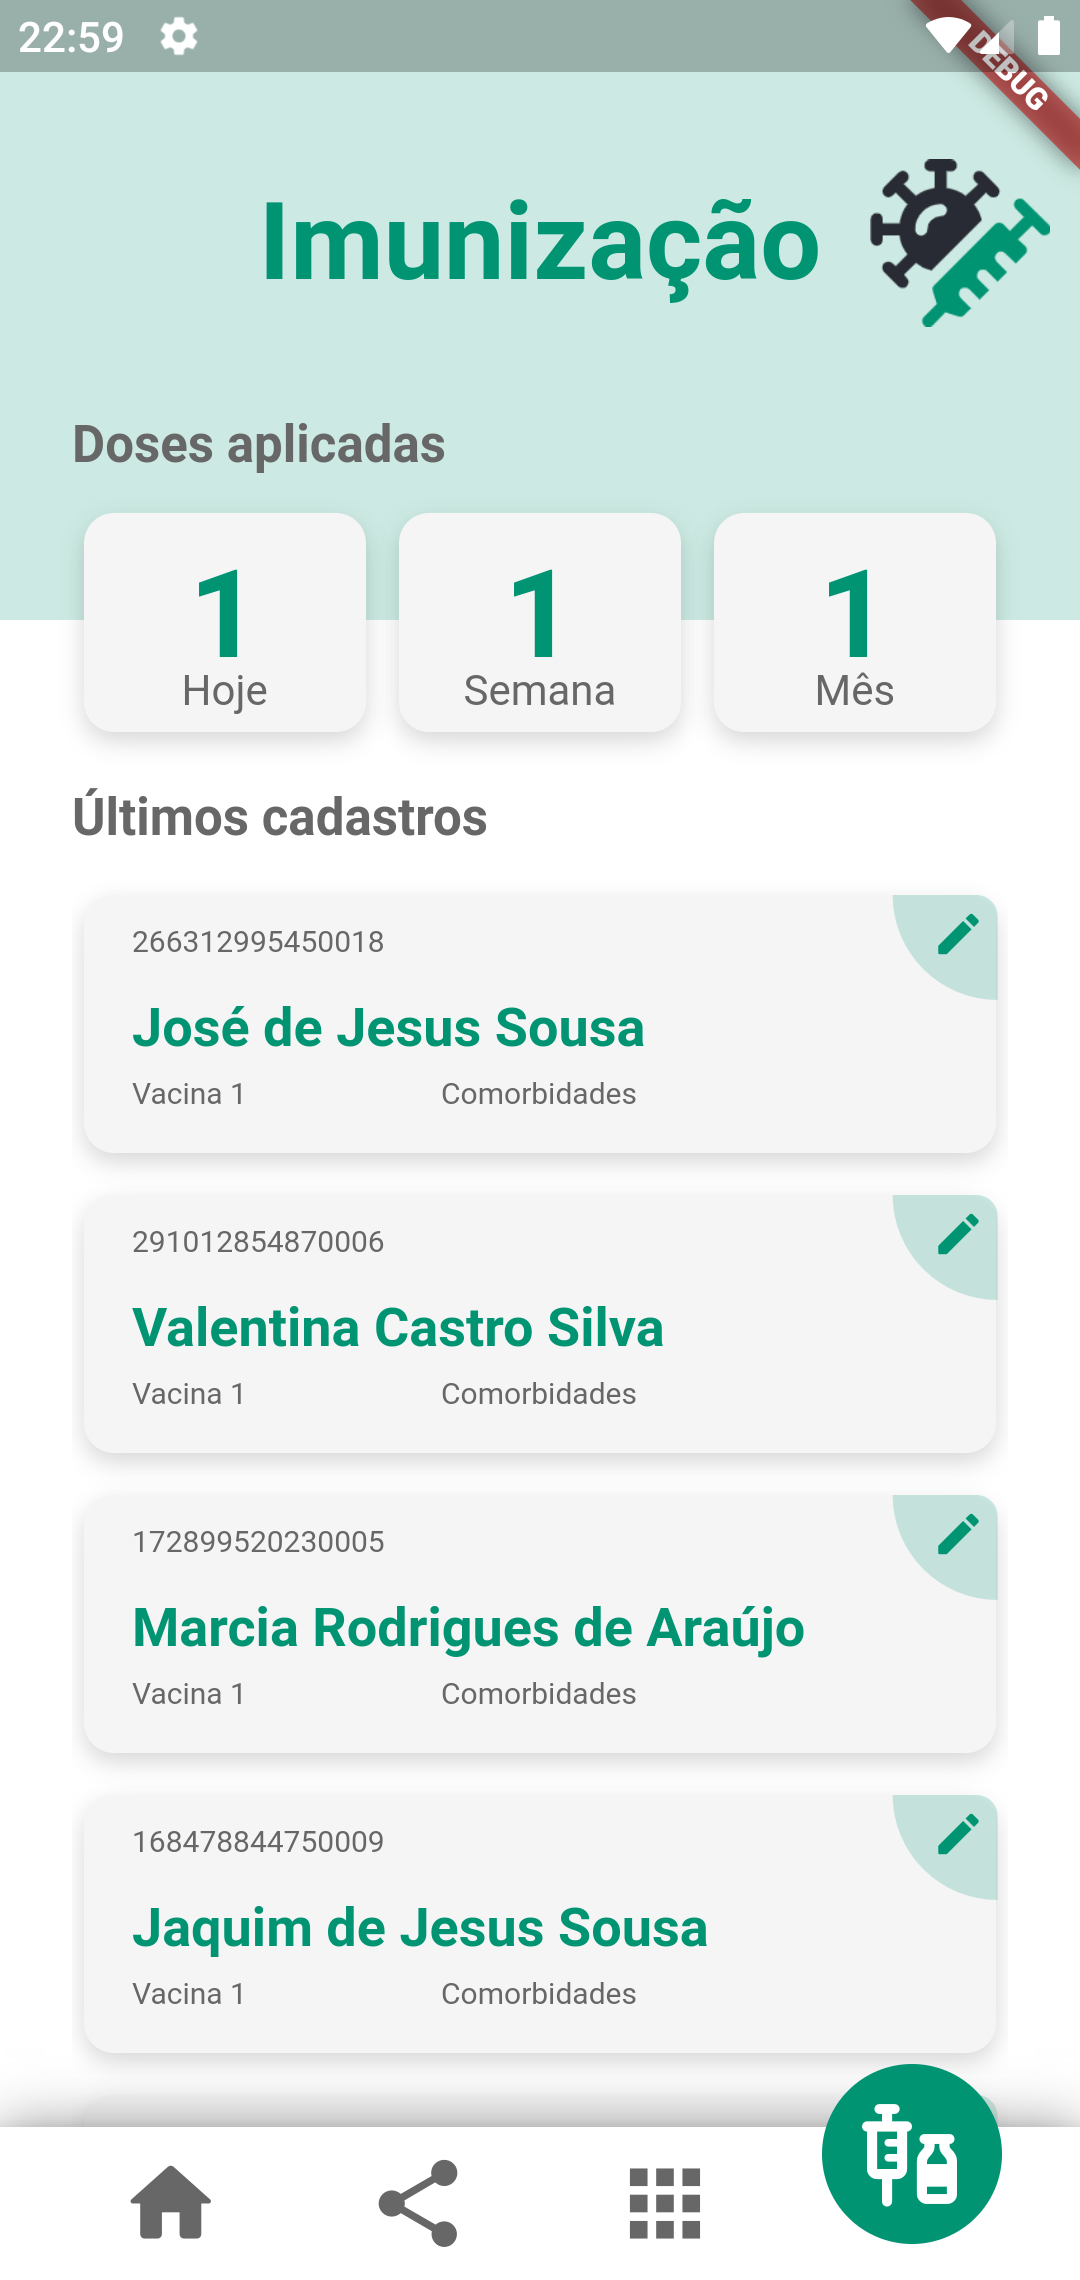
\includegraphics[width=0.29\columnwidth]{figuras/cap4/4_2_home_screen_2.png}}
            \qquad
          \subfloat[Tela \textbf{listagem de entidades}]{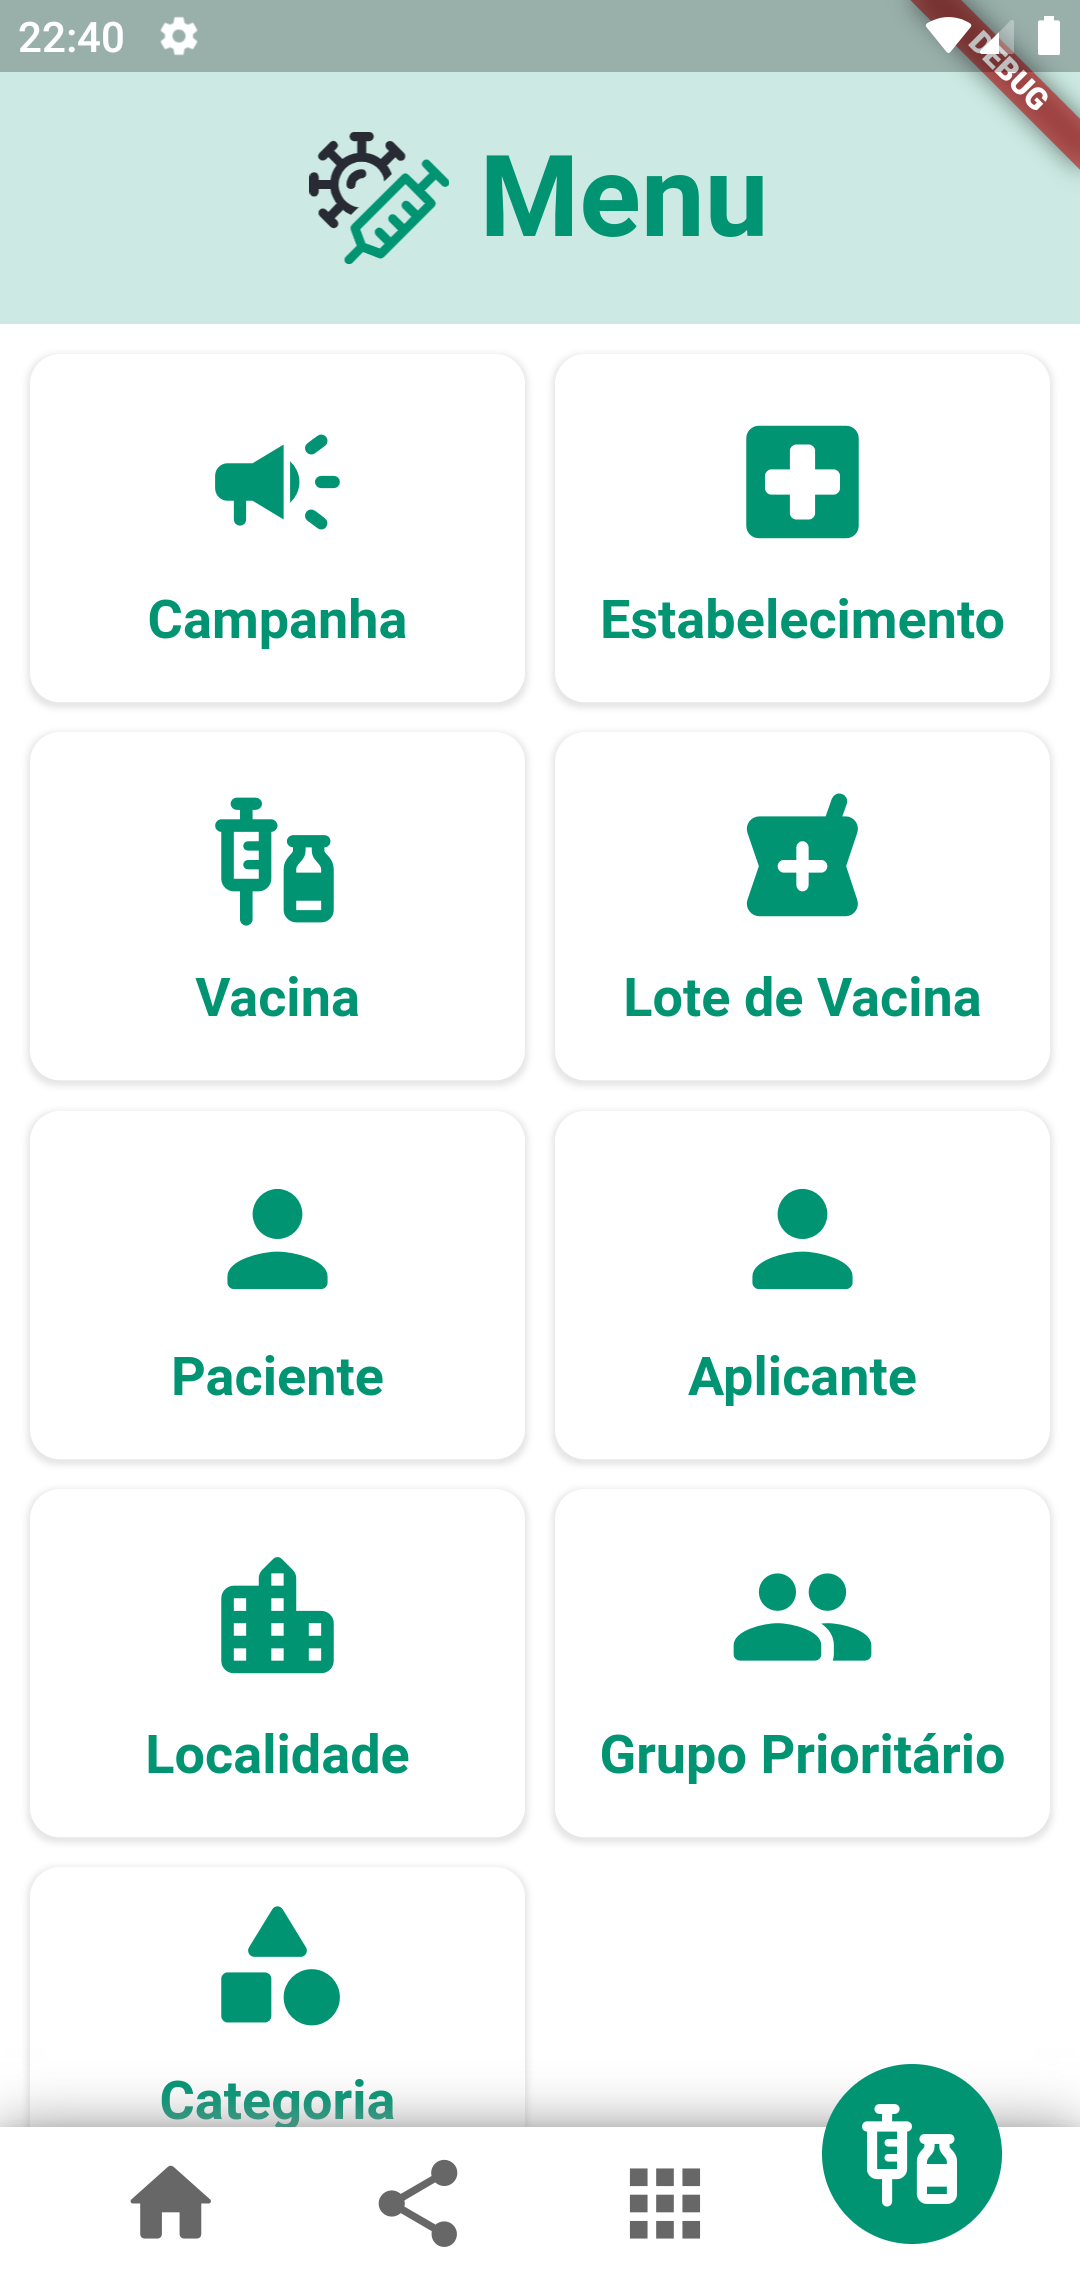
\includegraphics[width=0.29\columnwidth]{figuras/cap4/4_2_entities_screen.png}}
            \qquad
          \subfloat[Tela \textbf{exportação de dados}]{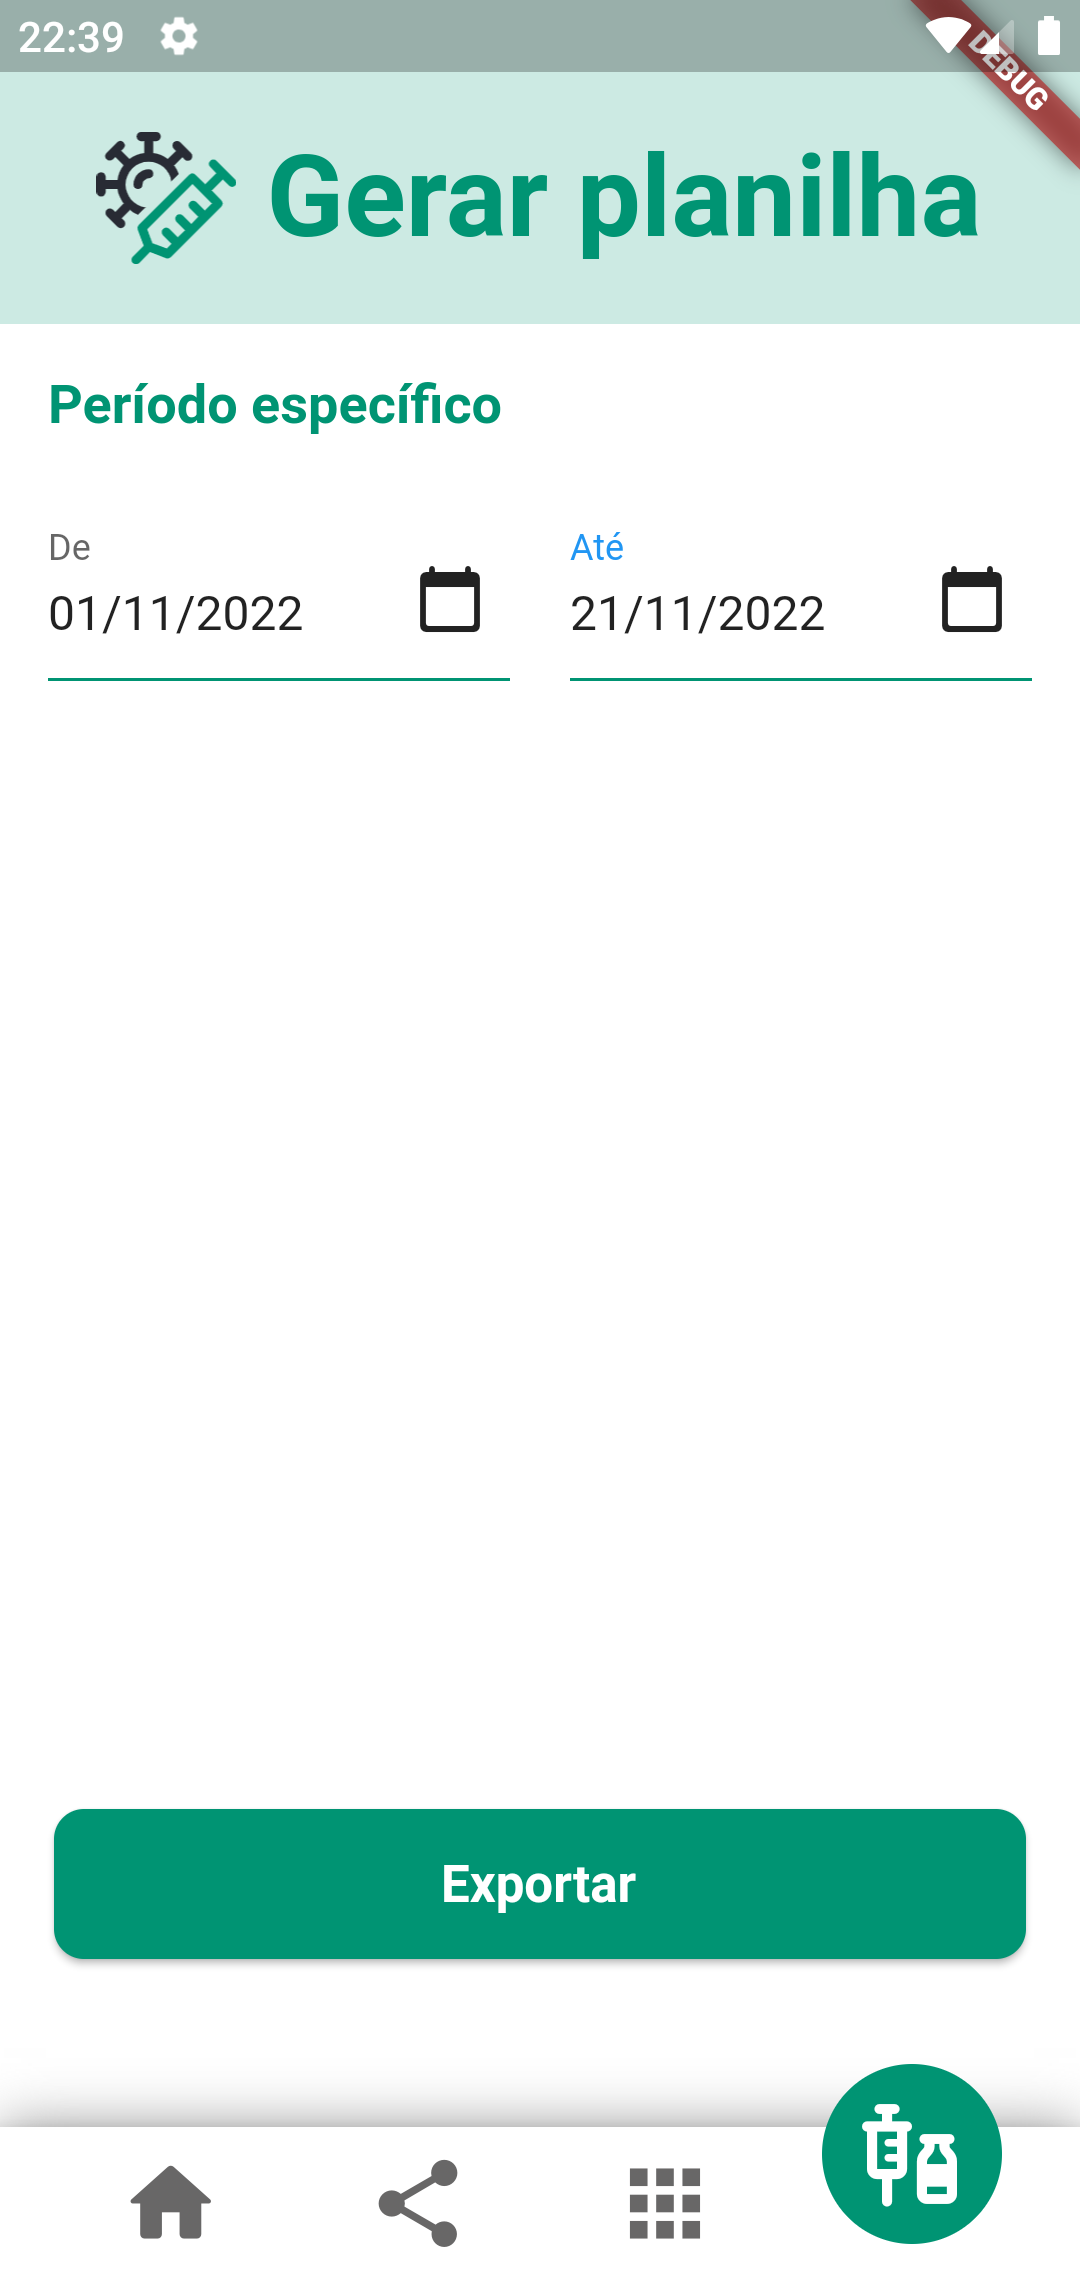
\includegraphics[width=0.29\columnwidth]{figuras/cap4/4_2_export_screen_4.png}}
    \caption[Principais telas da aplicação \textit{Nurse}]{Principais telas da aplicação \textit{Nurse}}
  % \fonte{Inserir autor aqui}
  
  \label{fig:nurse-main-screen}
\end{figure}

Todas as páginas apresentadas possuem um cabeçalho em verde que apresenta o título da página, um ícone da aplicação e, em alguns casos, um botão para voltar à página anterior. Além disso, as principais páginas possuem um rodapé que serve como sistema de navegação entre elas. Essa barra de navegação possui quatro ícones e cada um leva a uma página diferente. O primeiro ícone leva à página \textbf{Home}, o segundo à página de \textbf{listagem de entidades}, o terceiro à página de \textbf{exportação de dados} e o último e principal, ao conjunto de páginas de \textbf{cadastro de vacinação}. Essa última será apresentada em detalhes na seção \ref{cap5:SubSec:FluxoCadastroVacinacao}.

A página \textbf{Home} é a primeira página que o usuário visualiza quando abre o aplicativo. Nela, é possível ver o número de vacinas aplicadas no dia, na semana e no mês. Também é mostrado ao usuário a lista das últimas vacinas aplicadas e o paciente que as recebeu, além de outras informações sobre este.

A página \textbf{listagem de entidades} é a página que mostra ao usuário a lista de entidades cadastradas no aplicativo. Nela, é possível ver o nome da entidade e o 
ícone que a representa. Ao clicar em uma entidade, o usuário é levado à página de listagem daquela entidade.

Por fim, a página \textbf{exportação de dados} é a página que permite ao usuário exportar os dados do aplicativo referentes à vacinação para um arquivo \textbf{.csv}. Nela, o usuário pode filtrar o período que quer exportar os dados.


\begin{figure}[ht!]
  \centering
          \subfloat[Tela da lista de campanhas cadastradas]{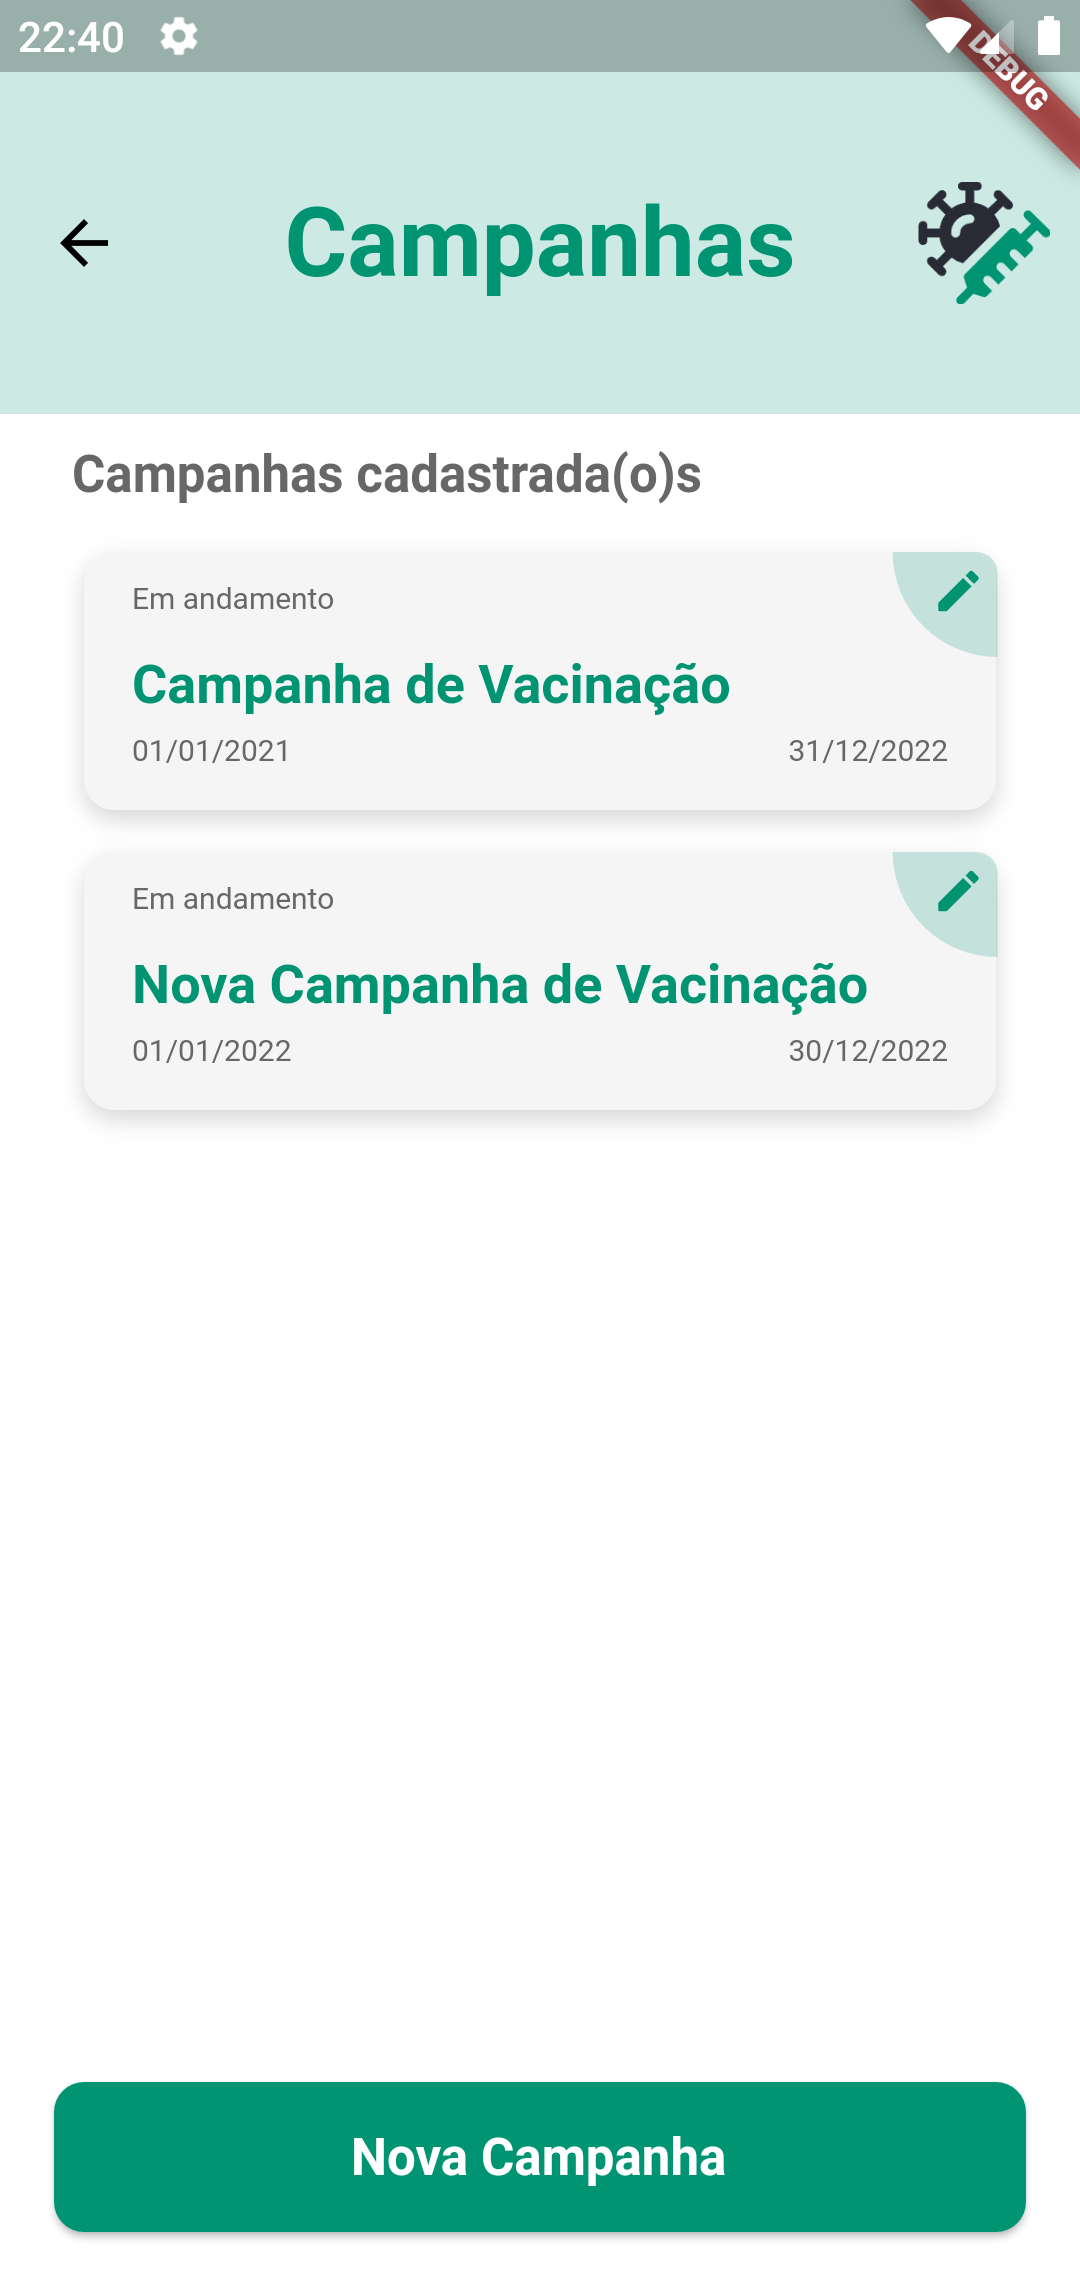
\includegraphics[width=0.29\columnwidth]{figuras/cap4/4_2_campaign_list_screen.png}}
            \qquad
          \subfloat[Tela de cadastro de nova campanha]{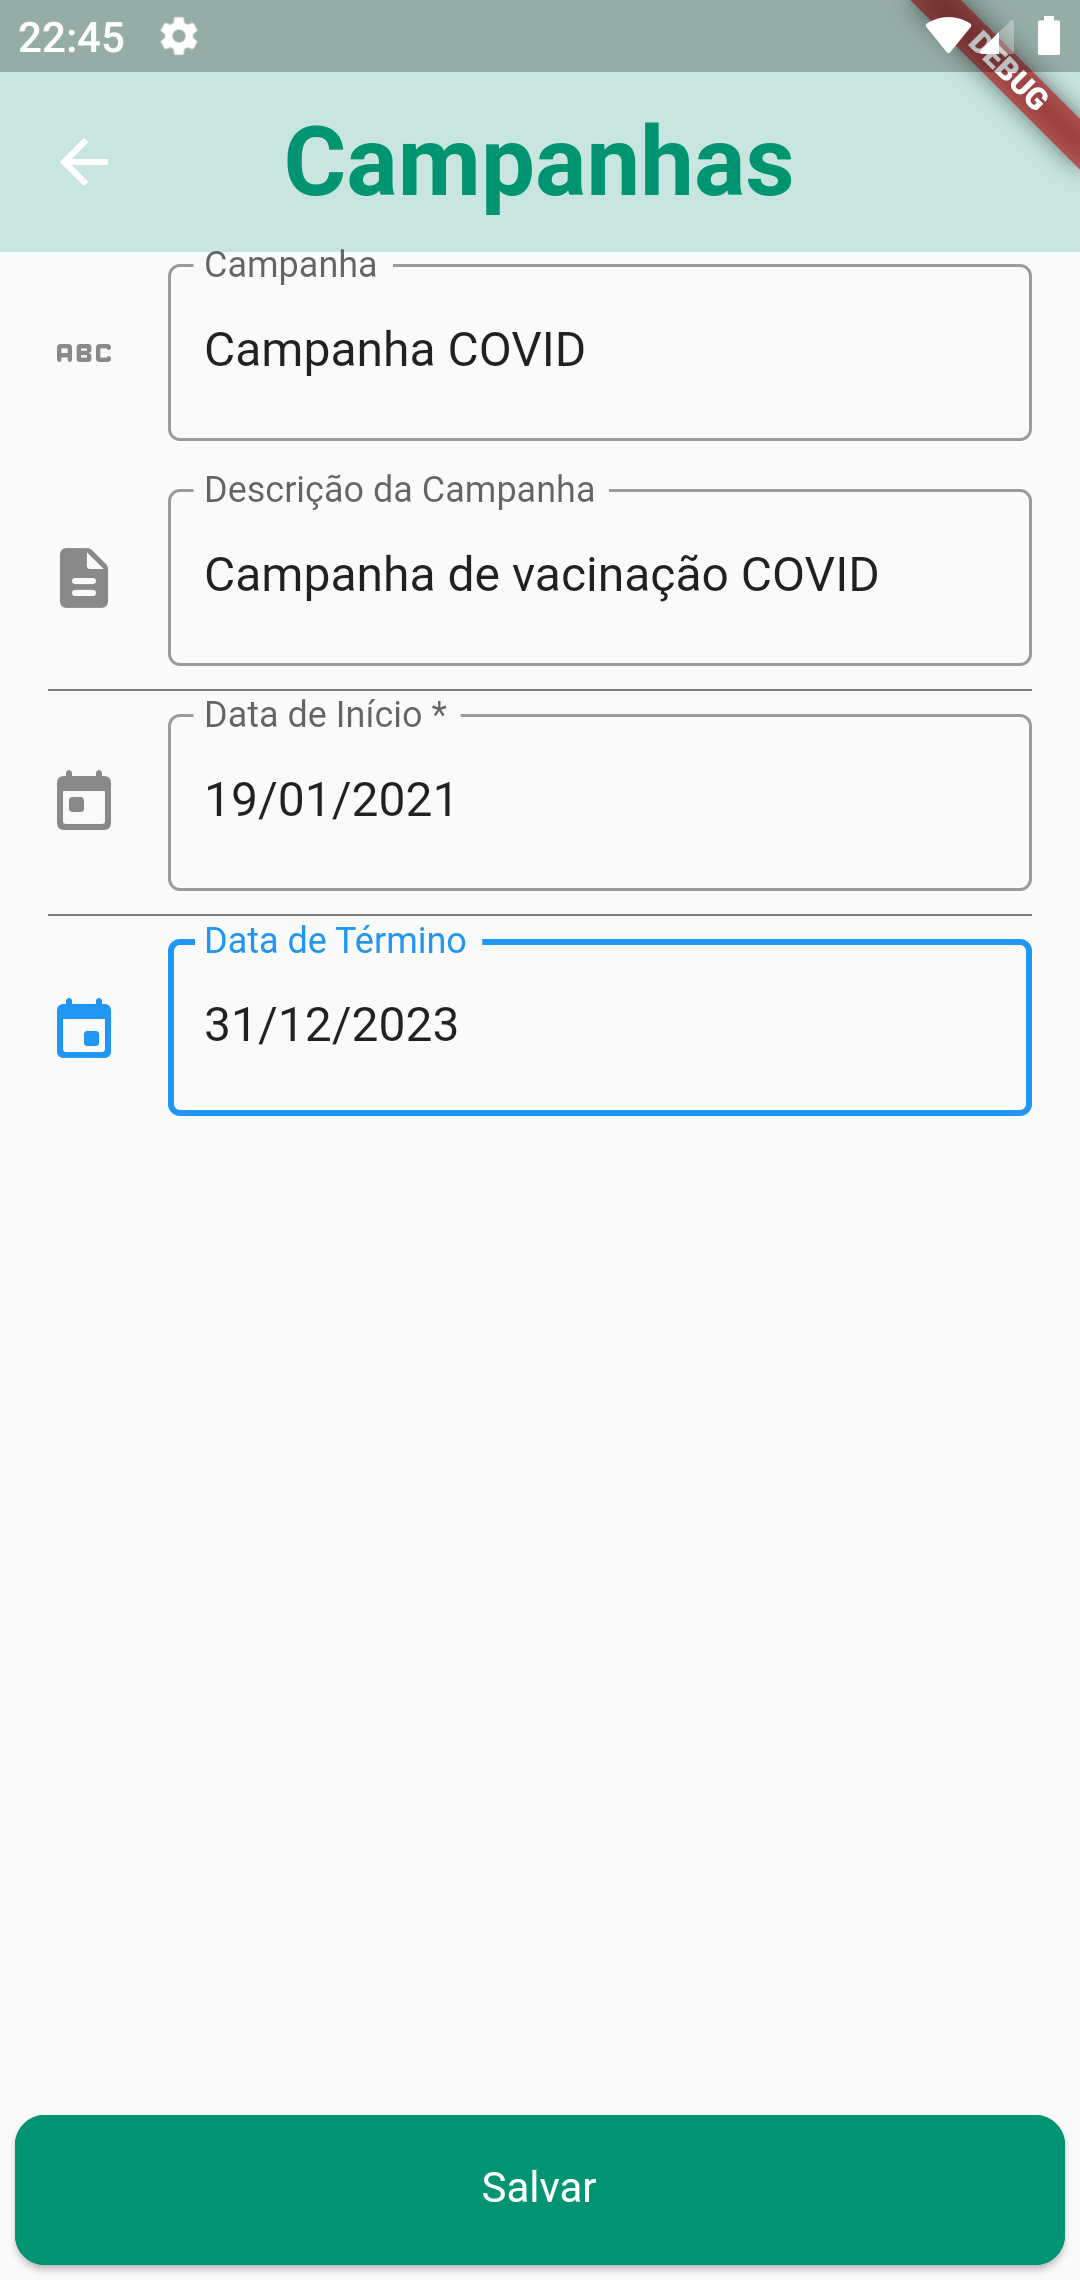
\includegraphics[width=0.29\columnwidth]{figuras/cap4/4_2_campaign_form_2.png}}
    \caption[Telas de listagem e cadastro de entidade]{Telas de listagem e cadastro de entidade}
  % \fonte{Inserir autor aqui}
  
  \label{fig:entity_list_new_entity}
\end{figure}

As telas da figura \ref{fig:entity_list_new_entity} apresentam um exemplo das telas que listam as campanhas cadastradas e o formulário de uma nova campanha. Na tela de listagem, pode-se ver duas campanhas cadastradas, um botão para novos cadastros na parte inferior na tela e um botão de edição em formato de lápis no canto superior direito de cada cartão. Esse cartão, por sua vez, apresenta as principais informações sobre aquela entidade. Por fim, quando quer-se editar um item, a página do formulário é iniciada com as informações previamente cadastradas daquele item.

\section{Pacotes e Bibliotecas}
\label{cap4:Sec:PacotesBibliotecas}

Nessa seção, serão apresentados os pacotes e bibliotecas utilizados no desenvolvimento do sistema. A tabela \ref{tab:packages}, presente no apêndice \ref{apendice:pacotes}, apresenta os pacotes utilizados no desenvolvimento do sistema e suas respectivas versões. Além dos pacotes principais, tem-se também os pacotes de desenvolvimento, que são utilizados apenas durante o desenvolvimento do sistema, como o \textit{flutter\_test} e o \textit{mobx\_codegen}, que são responsáveis pela criação de testes (ver seção \ref{cap5:Sec:TestesUnitarios}) e geração de arquivos relacionados ao gerenciamento de estado (ver seções \ref{cap2:Subsec:MobX}, \ref{cap4:SubSubSec:RegraNegocio} e \ref{cap4:Subsec:mobx-package}), respectivamente.

% [A revisar] nomes dos pacotes e bibliotecas 
Entre os pacotes e plugins utilizados, se destacam aqueles que estão relacionados com a persistência de dados (sqflite\_sqlcipher), com o gerenciamento de estado (mobx e flutter\_mobx), com a injeção de dependências (provider) e com a criação da planilha que será compartilhada (syncfusion\_flutter\_xlsio).

\subsection{\textit{Plugin}s \textit{sqflite\_sqlcipher} e \textit{sqflite}}
\label{cap4:Subsec:sqflite-sqlcipher-package}
O plugin \textit{sqflite} permite o uso do \textbf{SQLite} em aplicações \textit{Flutter} \cite{sqflite-package}. O \textit{sqflite\_sqlcipher}, por sua vez, adiciona ao primeiro a funcionalidade de criptografia do banco de dados através da biblioteca \textit{SQLCipher} \cite{sqlcipher-package}.

\subsection{Bibliotecas \textit{mobx} e \textit{flutter\_mobx}}
\label{cap4:Subsec:mobx-package}
O pacote \textit{mobx} é utilizado para a implementação do \textit{MobX} \ref{cap2:Subsec:MobX} nas aplicações em \textit{Dart/Flutter}. É com ele que o gerenciamento de estado segue o conceito de reatividade visto anteriormente, utilizando-se das suas principais classes: \textit{\textbf{Observable}}, responsável por criar o estado reativo da aplicação; e \textit{\textbf{Action}}, que definirá a função que muda esse estado. Além disso, para completar a tríade do MobX, este utiliza-se de um conjunto de reações, em forma de função, que são chamadas no momento em que o estado observado muda \cite{mobx-package}.

Em adição, têm-se o pacote \textit{flutter\_mobx}, o qual é responsável por implementar um \textit{widget} chamado \textit{\textbf{Observer}}. Este, por sua vez, garante que o seu \textit{widget} filho seja atualizado sempre que o estado relacionado a ele mude. O \textit{Observer} também é um representante das reações do MobX que, nesse caso, reage atualizando a interface do usuário \cite{flutter-mobx-package}.

No desenvolvimento da classe \textbf{HomeController}, a qual gerencia o estado observado pelos componentes da página \textbf{Home}, utilizou-se as classes \textbf{Action}, para definir a função responsável por alterar o estado observável, e \textbf{ObservableList}, uma variante da classe \textbf{Observable} para listas.

\begin{lstlisting}[caption={Uso do \textit{MobX} na classe \textbf{HomeController}}, label={lst:home_controller_mobx}]
  class HomeController {
    final ApplicationRepository applicationRepository;

    final applications = ObservableList<Application>.of(
      List<Application>.empty(growable: true),
    );

    late final fetchApplications = Action(getApplications);

    HomeController() : applicationRepository = DatabaseApplicationRepository() {
      fetchApplications();
    }

    Future<List<Application>> getApplications() async {
      final result = await applicationRepository.getApplications();
      applications.clear();
      applications.addAll(result.reversed);

      return applications;
    }

    /*...*/
  }
\end{lstlisting}

A propriedade \textit{applications} recebe, inicialmente, um \textbf{ObservableList} vazio do tipo \textit{Application} e a função \textit{fetchApplications} foi definida como a ação que modifica o estado observável, isto é, a lista de aplicações. A ação é chamada no construtor da classe \textbf{HomeController} para que a lista de aplicações seja preenchida assim que a classe for instanciada. Essa lista, por sua vez, é preenchida quando a busca realizada pela classe \textbf{ApplicationRepository} no banco de dados finaliza com sucesso.  A função \textit{fetchApplications} é chamada, também, toda vez que o usuário finaliza um novo cadastro de aplicação de vacina e é redirecionado novamente à tela inicial \textbf{Home}.

\begin{lstlisting}[caption={Uso do \textit{MobX} no \textit{widget} \textbf{Home}}, label={lst:home_page_mobx}]
  class Home extends StatelessWidget {
    /*...*/

    @override
    Widget build(BuildContext context) {
      return Scaffold(
        
        /*...*/
      
        floatingActionButton: VaccinationButton(
          newPage: "/vaccinations/new",
          onCallback: () => context.read<HomeController>().
          fetchApplications(),
        ),
        
        /*...*/

      );
    }
  }
\end{lstlisting}

No código que define a classe \textbf{Home}, mostrada parcialmente no trecho de código \ref{lst:home_page_mobx}, têm-se o \textit{widget} \textbf{Scaffold}, o qual possui a propriedade \textbf{\textit{floatingActionButton}}, que recebe o \textit{widget} \textbf{VaccinationButton}. A sua propriedade \textit{onCallback} recebe uma função que chama \textit{fetchApplications} da classe \textbf{HomeController}, para que a lista de aplicações seja atualizada. A forma como o estado é injetado na classe \textbf{Home} é explicado adiante, na \ref{cap4:Subsec:Provider}.

\subsection{Pacote \textit{provider}}
\label{cap4:Subsec:Provider}
Como descrito anteriormente, na \ref{cap2:Subsec:Provider}, o estado pode ser injetado em qualquer \textit{widget} por meio do \textit{Provider}. Sendo assim, utilizou-se o \textit{Provider} nesse projeto não para gerenciamento do estado diretamente, mas para injetar o estado gerenciado pelo \textit{mobx} em qualquer \textit{widget} da aplicação. Para isso, foi utilizado o pacote \textit{provider} \cite{provider-package}.

Desse pacote, utilizou-se duas estratégias principais:
\begin{itemize}
  \item \textbf{Provider.of<T>(context)}: injeta a classe T a partir do contexto passado via parâmetro. O Provider, então, busca na árvore de \textit{widgets} acima do \textit{widget} atual a instância mais próxima da classe T \cite{provider-package}. A seguir, no trecho de código \ref{lst:appliers_page_provider}, tem-se um exemplo de uso dessa estratégia.
  \item \textbf{context.read<T>().fn()}: assim como o anterior, utiliza-se do contexto para buscar a classe T desejada e, em seguida, faz uma chamada da função denominada \textit{fn} no exemplo, mas não passa a observar as mudanças de estado que ocorrem nessa classe, diferentemente da função \textit{watch} \cite{provider-package}. Um exemplo do seu uso foi apresentado no trecho de código \ref{lst:home_page_mobx}, no qual \textit{fetchApplications} representa a função \textit{fn} aqui descrita.
\end{itemize}

\begin{lstlisting}[caption={Uso do \textit{Provider} no \textit{widget} \textbf{Appliers}}, label={lst:appliers_page_provider}]
  class Appliers extends StatelessWidget {
    const Appliers({Key? key}) : super(key: key);

    @override
    Widget build(BuildContext context) {
      final controller = Provider.of<AppliersPageController>(context);
      /*...*/

      return EntityList<Applier>(
        title: "Aplicantes",
        controller: controller,
        /*...*/
      );
    }
  }
\end{lstlisting}

\subsection{Biblioteca Excel (XlsIO)}
\label{cap4:Subsec:syncfusion_flutter_xlsio}
Utilizando-se do pacote \textit{syncfusion\_flutter\_xlsio}, foi possível gerar um arquivo \textit{.xlsx} a partir de uma lista de aplicações de vacina. Para isso, criou-se uma classe chamada \textbf{ExcelService} que possui dois métodos públicos: \textbf{\textit{shareExcelFile}} e \textbf{\textit{openExcelFile}}. Cada um desses métodos é chamado quando o usuário segue o fluxo apresentado na figura \ref{fig:export_flux_2} e descrito em detalhes na seção \ref{cap5:SubSec:FluxoExportacao}.

O método \textbf{\textit{shareExcelFile}} cria um arquivo \textit{.xlsx} e permite que o usuário o compartilhe, enquanto o método \textbf{\textit{openExcelFile}} cria um arquivo \textit{.xlsx} e o abre no aplicativo de planilhas do usuário. A seguir, na figura \ref{fig:excel_service_diagram}, tem-se o fluxo de execução de ambos os métodos dentro da classe \textbf{ExcelService}.

\begin{figure}[!ht]
  \centering
  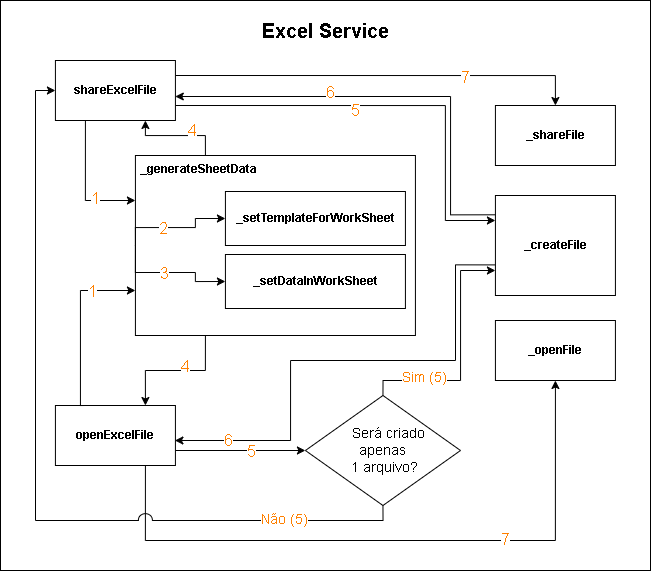
\includegraphics[width=\textwidth]{figuras/cap4/4_3_4_excel_service_diagram.png}
  \caption{Descritivo de fluxo dos métodos da classe \textbf{ExcelService}}
  \label{fig:excel_service_diagram}
\end{figure}

A ordem de execução dos métodos segue a ordem das setas numeradas. Cada um dos métodos é descrito a seguir:

\begin{itemize}
  \item \textbf{Etapa 1}: os métodos \textbf{\textit{shareExcelFile}} e \textbf{\textit{openExcelFile}} recebem como parâmetros a lista das aplicações cadastradas e o período de tempo que o usuário deseja exportar ou visualizar. Estas informações são, então, organizadas em um mapa de datas e aplicações e enviadas ao método \textbf{\textit{\_generateSheetData}}
  \item Etapas \textbf{2} e \textbf{3}: o método \textbf{\textit{\_generateSheetData}} recebe como parâmetro o mapa de datas e aplicações. A partir dos métodos \textbf{\textit{\_setTemplateForWorkSheet}} e \textbf{\textit{\_setDataInWorkSheet}}, um objeto do tipo \textbf{\textit{Workbook}} é, respectivamente estruturado e preenchido com os dados recebidos. Esse \textbf{\textit{Workbook}} é, então transformado em uma lista de bytes por meio de seu método interno \textbf{\textit{Workbook.saveAsStream()}}. Por fim, cada agrupamento de bytes é retornado em um novo mapa, onde a chave é a data das aplicações e o valor é um outro mapa de doses aplicadas e agrupamento de bytes.
  \item \textbf{Etapa 4}: o método \textbf{\textit{\_generateSheetData}} retorna o agrupamento de bytes para as funções \textbf{\textit{shareExcelFile}} ou \textbf{\textit{openExcelFile}}, a depender de qual fluxo está sendo executado, e cada um desses agrupamentos será processado individualmente, como se segue.
  \item \textbf{Etapa 5}: para o método \textbf{\textit{openExcelFile}}, será verificado a quantidades de agrupamentos retornados. Caso seja apenas um, o arquivo será criado a partir desse agrupamento e passará ao próximo passo. Caso contrário, o fluxo desse método será finalizado e os dados serão redirecionados ao método \textbf{\textit{shareExcelFile}}. Já para este último, o fluxo é direto e cada cada conjunto de bytes separados por datas de aplicação e doses aplicadas será salvo em um arquivo.
  \item \textbf{Etapa 6}: considerando que o fluxo dos métodos \textbf{\textit{shareExcelFile}} e \textbf{\textit{openExcelFile}} foi o mesmo, ou seja, a criação dos arquivos na função \textbf{\textit{\_createFile}}, o(s) arquivo(s) recebido(s) será(ão) enviados de volta para as funções principais.
  \item \textbf{Etapa 7}: Por fim, o método \textbf{\textit{shareExcelFile}} chama a função \textbf{\textit{\_shareFile}} para compartilhar o arquivo gerado, enquanto o método \textbf{\textit{openExcelFile}} chama a função \textbf{\textit{\_openFile}} para abrir o arquivo gerado. Ambas as funções são descritas a seguir.
\end{itemize}

A função \textbf{\textit{\_shareFile}} recebe como parâmetro o arquivo gerado e, a partir da biblioteca \textit{share\_plus} e do seu método \textbf{\textit{Share.shareFiles}}, permite que o usuário compartilhe o arquivo gerado \cite{share_plus-package}. A função \textbf{\textit{\_openFile}}, por sua vez, também recebe o arquivo gerado de forma análoga à primeira função e, a partir da biblioteca \textit{open\_file} e do seu método \textbf{\textit{OpenFile.open}}, realiza a chamada a uma aplicação que possa abrir um arquivo no formato \textit{.xlsx}.

\section{Persistência de Dados}
\label{cap4:Sec:PersistenciaDados}
A persistência de dados, como descrita na seção \ref{cap2:Sec:PersistenciaDados}, é realizada por meio de um banco de dados relacional, o \textit{SQLite}. A biblioteca \textit{sqflite} é utilizada para a comunicação com o banco de dados \cite{sqflite-package}. A estrutura do banco de dados da aplicação como ela foi implementada é descrita nesta seção.

\subsection{Diagrama de Classes}
\label{cap4:SubSec:DiagramaClasses}
Foram definidas 9 entidades (ou classes) para a aplicação \textbf{Nurse}, as quais foram agrupadas em 3 macro-grupos: \textbf{Paciente}, \textbf{Vacinação} e \textbf{Infraestrutura}. Cada uma dessas entidades possui um identificador único, chamada chave primária (do inglês, \textit{Primary Key} (PK)) e algumas delas possuem uma ou mais chaves estrangeiras (do inglês, \textit{Foreign Key} (FK)) \cite{heuser09banco}. Além disso, cada entidade possui um ou mais atributos, que são apresentados na figura \ref{fig:diagrama_classes} e descritos a seguir.

\begin{figure}[!ht]
  \centering
  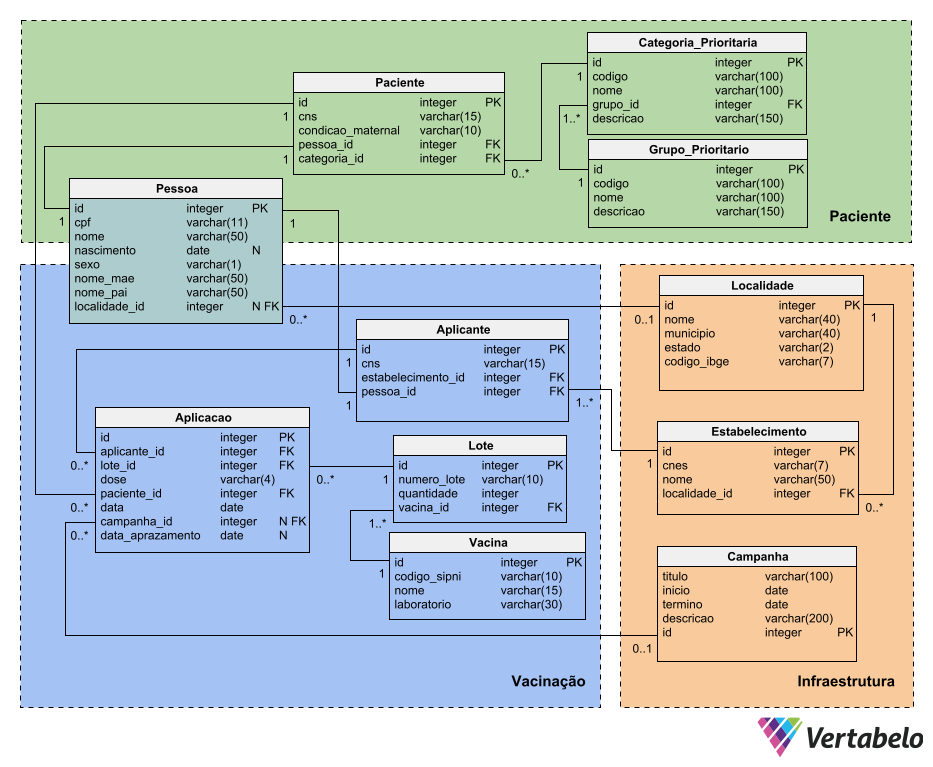
\includegraphics[width=\textwidth]{figuras/cap4/4_4_1_diagrama_classes.png}
  \caption{Diagrama de classe para a aplicação \textbf{Nurse}}
  \label{fig:diagrama_classes}
\end{figure}

\begin{itemize}
  \item \textbf{Pessoa}: é a entidade que representa uma pessoa, seja ela um paciente ou um profissional de saúde. Essa entidade possui os atributos \textbf{nome}, \textbf{cpf}, \textbf{data de nascimento}, \textbf{sexo}, \textbf{nome da mãe}, \textbf{nome do pai} e \textbf{localidade} onde reside. Essa entidade faz parte de dois grupo distintos: grupo 'Paciente' e grupo 'Aplicação', pois ela pode estar associada a um paciente ou a um aplicante da vacina.
  \item Grupo \textbf{Paciente}
  \begin{itemize}
    \item \textbf{Paciente}: é a entidade que representa um paciente. Essa entidade possui os atributos \textbf{cns} (número do Cartão Nacional de Saúde) e \textbf{condição maternal}. Além disso, a entidade \textbf{Paciente} possui duas chaves estrangeiras para as entidades \textbf{Pessoa} e \textbf{Categoria Prioritária}.
    \item \textbf{Categoria Prioritária}: é a entidade que representa uma categoria prioritária do paciente. Essa entidade possui os atributos \textbf{nome}, \textbf{código} e \textbf{descrição}. Além disso, a entidade \textbf{Categoria Prioritária} possui uma chave estrangeira para o seu \textbf{Grupo Prioritário}.
    \item \textbf{Grupo Prioritário}: é a entidade que representa um conjunto de categorias prioritárias. Um exemplo de grupo é 'Faixa Etária' e as categorias desse grupo são subconjuntos de idades (pessoas com mais de 60 anos, pessoas com menos de 18 anos etc...). Essa entidade possui os atributos \textbf{nome}, \textbf{código} e \textbf{descrição}.
  \end{itemize}
  \item Grupo \textbf{Infraestrutura}
  \begin{itemize}
    \item \textbf{Localidade}: é a entidade que representa uma localidade, seja ela uma comunidade ou uma cidade. Essa entidade possui os atributos \textbf{nome da localidade}, \textbf{município}, \textbf{estado} e \textbf{código do IBGE}.
    \item \textbf{Estabelecimento}: é a entidade que representa um estabelecimento de saúde. Essa entidade possui os atributos \textbf{nome} e \textbf{CNES} (Cadastro Nacional de Estabelecimentos de Saúde). Além disso, a entidade \textbf{Estabelecimento} possui uma chave estrangeira para a entidade \textbf{Localidade}.
    \item \textbf{Campanha}: é a entidade que representa uma campanha de vacinação. Essa entidade possui os atributos \textbf{título}, datas de \textbf{início} e \textbf{término} da campanha e sua \textbf{descrição}.
    % ref da sigla CNES: https://cnes.datasus.gov.br/ 21/11/2022 
  \end{itemize}
  \item Grupo \textbf{Vacinação}
  \begin{itemize}
    \item \textbf{Aplicante}: é a entidade que representa o profissional de saúde que realizou a aplicação da vacina no paciente. Essa entidade possui o atributo \textbf{cns}, assim como o paciente. Além disso, a entidade \textbf{Aplicante} possui duas chaves estrangeiras para as entidades \textbf{Pessoa} e \textbf{Estabelecimento}.
    \item \textbf{Vacina}: é a entidade que representa o agente imunizante que será aplicado no paciente. Essa entidade possui os atributos \textbf{nome} da vacina, seu \textbf{código SI-PNI} e o \textbf{laboratório} do fabricante.
    \item \textbf{Lote}: é a entidade que representa um lote de vacinas. Essa entidade possui os atributos \textbf{número do lote} e \textbf{quantidade de vacinas} no lote. Além disso, a entidade \textbf{Lote} possui uma chave estrangeira para a entidade \textbf{Vacina}.
    \item \textbf{Vacinação}: é a entidade central da aplicação. Ela representa todo o conjunto de informações que estão associadas ao ato de vacinar. Seus atributos representam essa centralidade. São eles: \textbf{Aplicante}, \textbf{Lote da vacina}, \textbf{Paciente} e \textbf{Campanha de vacinação}, as quais são todas chaves estrangeiras para outras tabelas. Além disso, a entidade \textbf{Vacinação} possui os atributos \textbf{dose da vacina}, \textbf{data de aplicação} e \textbf{data prazo} para próxima aplicação.
  \end{itemize}
\end{itemize}

Alguns desses atributos são obrigatórios, como o \textbf{cpf} e o \textbf{nome}, já outros podem ser deixados nulos, como é o caso do campo \textbf{sexo}, todos da tabela \textbf{Pessoa}. Além dessa, a tabela \textbf{Aplicação} também possui dois atributos chamados anuláveis, que são o identificador da tabela \textbf{Campanha} e o atributo \textbf{data de aprazamento}.

\subsection{Uso do Banco de Dados}
\label{cap4:Sec:UsoBancoDados}
O banco de dados é gerenciado pela classe \textbf{DatabaseManager}. Essa classe possui o método público \textbf{tryToInit}, que é chamado logo na inicialização do app \textbf{Nurse} e é responsável por abrir o banco de dados ou criá-lo quando este ainda não existe. Uma vez aberto, a classe \textbf{DatabaseManager} é responsável por gerenciar as requisições de inserção, atualização e/ou consulta realizadas pelo usuário. Isso é possível por meio da interface \textbf{DatabaseInterface} e do objeto \textbf{Database}, que define os métodos de acesso ao banco de dados e envia os comandos sql para o banco, respectivamente.















% \begin{algorithm}
% %% \SetLine
% \Entrada{$x$: vetores de valores; $y$ = $L(x)$; $p$: valor de entrada a ser calculado }
% \Saida{$s$ = $L(p)$}
% $n \leftarrow \mathtt{comprimento}(x)$\;
% $s \leftarrow 0$\;
% \Para {$i=1$ \Ate $n$} {
% 	$L \leftarrow 1$\;
% 	\Para {$j=1:1:n$} {
% 		\Se{$i \neq j$} {
% 			$L \leftarrow L* \left( \dfrac{p-x[j]}{x[i]-x[j]} \right) $
% 		}
% 	}
% 	$s \leftarrow s + L*y[i]$\;
% }
% \Retorna $s$\;
% \caption{Algoritmo para interpolação de Lagrange.}
% \label{algo:1}
% \end{algorithm}

% \begin{algorithm}
% %% \SetLine
% \Entrada{$a$: valor inicial; $b$: valor final; $n$: número de subintervalos (deve ser múltiplo de 2)  }
% \tcc{A função a ser integrada é definida em uma função denominada \texttt{f}, fora do escopo deste algoritmo.}
% \Saida{$I$ = integral de \texttt{f} entre $a$ e $b$}
% $h \leftarrow$ $\dfrac{b-a}{n}$\;
% $x[1] \leftarrow a$\;
% $y[1] \leftarrow f(a)$\;
% $I \leftarrow 0$\;
% $k \leftarrow 2$\;
% \Enqto {$k <= n$} {
% 	$x[i] \leftarrow x[i-1] + h$\;
% 	$y[i] \leftarrow f(x[i])$\;
% 	\eSe{$i \% 2 = 0$} {
% 		$I \leftarrow I + 4*y[i]$\;
% 	}
% 	{
% 		$I \leftarrow I + 2*y[i]$\;
% 	}
% 	$k = k+1$\;
% }
% $x[n+1] \leftarrow b$\;
% $y[n+1] \leftarrow f(x[i+1])$\;
% $I \leftarrow I + \dfrac{h}{3}*(I + y[n+1])$\;
% \Retorna $I$\;
% \caption{Algoritmo para a integração pelo primeiro método de Simpson.}
% \label{algo:2}
% \end{algorithm}


% Cap. 5 - Experimentos e Resultados
%%
%% Capítulo 5: Experimentos e Resultados
%%

\mychapter{Experimentos e Resultados}
\label{Cap:ExperimentosResultados}

Posso escrever sobre os testes feitos
Escrever sobre os fluxos possíveis no sistema. Entrada de dados, mudanças de telas e saída de dados.

\section{Testes Unitários}
\label{cap5:Sec:TestesUnitarios}
Mostrar a cobertura de testes unitários do sistema.

\section{Testes de Performance}
\label{cap5:Sec:TestesPerformance}
Buscar os métodos de testes de performance do Flutter e do Dart.

\section{Fluxos de Telas}
\label{cap5:Sec:FluxosTelas}
Mostrar os principais fluxos de telas do sistema.

\subsection{Fluxo de cadastro de entidade}
\label{cap5:SubSec:FluxoCadastroEntidade}
Mostrar o fluxo de compartilhamento de dados em planilha.

\subsection{Fluxo de cadastro de vacinação}
\label{cap5:SubSec:FluxoCadastroVacinacao}
Mostrar o fluxo de compartilhamento de dados em planilha.

\subsection{Fluxo de exportação}
\label{cap5:SubSec:FluxoExportacao}
Mostrar o fluxo de compartilhamento de dados em planilha.

\section{Testes de segurança}
\label{cap5:Sec:TestesSeguranca}
Aqui posso falar sobre a tentativa de adicionar dados inválidos.







% Cap. 6 - Conclusão
%%
%% Capítulo 5: Conclusões
%%

\mychapter{Conclusão}
\label{Cap:Conclusao}

% Escrever sobre o que espero para o futuro da aplicação.
%   - Melhorar a interface gráfica (responsividade, usabilidade, adaptatividade e acessibilidade)
%   - Melhorar a segurança (autenticação, autorização, criptografia e integridade)
%   - Melhorar a performance (velocidade de resposta, escalabilidade e disponibilidade)
%   - Melhorar a manutenibilidade (testabilidade, documentação e reutilização)
%   - Melhorar a qualidade (padronização, estabilidade e confiabilidade)
%   - Adicionar animações e transições para tornar o app mais fluído e agradável durante seu uso.

% Escrever quais os meus erros e como corrigi-los.


% Referências bibliográficas (geradas automaticamente)
% Aqui, o comando \phantomsection é utilizado para auxiliar o pacote "hyperref" a fazer a
% referência correta dos links das referências bibliográficas com a página respectiva.
% Caso seja tirado, o "hyperref" irá apontar o link das referências bibliográficas para a
% última subseção da conclusão.
\phantomsection
\addcontentsline{toc}{chapter}{Referências bibliográficas}
\bibliography{bibliografia/bibliografia}

\appendix

%Apêndice A
%%
%% Apêndice 1: Requisitos funcionais detalhados
%%

\mychapter{Requisitos funcionais detalhados}
\label{apendice:requisitos_funcionais_detalhados}

\rowcolors{1}{white}{green!10}
\begin{longtable}{
  | >{\centering}m{0.10\textwidth} 
  | >{\centering}m{0.30\textwidth} 
  | m{0.60\textwidth} |}
  
    \hline
    \rowcolor{green!100}
    \textbf{Código} & \textbf{Requisito} & \textbf{Descrição} \\ \hline \hline
    \textbf{RF01}  &  \textbf{Cadastrar entidades} & \textbf{Permitir que o usuário cadastre novas entidades}  \\ \hline \hline
    RF01-01 & Cadastrar Vacinações              & Fornecer para preenchimento os campos obrigatórios aplicante, estabelecimento de aplicação, vacina, lote, informações do paciente (pré-cadastrado ou não), dose e data da aplicação da vacina e os campos opcionais campanha da vacinação que está sendo efetuada e data da próxima vacina \\ \hline
    RF01-02 & Cadastrar Campanhas               & Fornecer para preenchimento os campos obrigatórios título e datas de início de fim e o campo opcional descrição da campanha  \\ \hline
    RF01-03 & Cadastrar Estabelecimentos        & Fornecer para preenchimento os campos obrigatórios nome, CNES e endereço do estabelecimento de saúde \\ \hline
    RF01-04 & Cadastrar Vacinas                 & Fornecer para preenchimento os campos obrigatórios nome, fabricante e código da vacina \\ \hline
    RF01-05 & Cadastrar Lotes de Vacina         & Fornecer para preenchimento os campos obrigatórios código, nome e quantidade de doses da vacina no lote \\ \hline
    RF01-06 & Cadastrar Pacientes               & Fornecer para preenchimento os campos obrigatórios CNS, CPF, nome, data de nascimento, localidade, categoria prioritária e condição maternal e os campos opcionais sexo e nomes do pai e da mãe do paciente \\ \hline
    RF01-07 & Cadastrar Aplicantes              & Fornecer para preenchimento os campos obrigatórios CNS, CPF, nome, localidade e estabelecimento de saúde de atuação e os campos opcionais data de nascimento, sexo e nomes do pai e da mãe do paciente \\ \hline
    RF01-08 & Cadastrar Localidades             & Fornecer para preenchimento os campos obrigatórios código do IBGE, nome, cidade e estado da localidade \\ \hline
    RF01-09 & Cadastrar Grupos Prioritários     & Fornecer para preenchimento o campo obrigatório código e os campos opcionais nome e descrição do grupo prioritário \\ \hline
    RF01-10 & Cadastrar Categorias Prioritárias & Fornecer para preenchimento os campos obrigatórios* código e grupo prioritário pertencente e os campos opcionais nome e descrição da categoria prioritária \\ \hline
    RF01-11 & Botão de salvamento               & Fornecer para preenchimento os campos obrigatórios* botão para salvamento dos dados cadastrados em todos os formulários \\ \hline

  \hiderowcolors
  \caption{Requisitos funcionais da aplicação Nurse: detalhes do requisito RF01}
  \label{tab:rf01_detalhe}
\end{longtable}

% \begin{table}[ht!]
%   \centering
%   {\rowcolors{0}{white}{green!10}
%   \begin{tabularx}{\textwidth}{
%     | >{\centering\arraybackslash}m{0.10\textwidth} 
%     | >{\centering\arraybackslash}X 
%     | >{\raggedright\arraybackslash}X | }
%     \hline
%     \rowcolor{green!100}
%     \textbf{Código} & \textbf{Requisito} & \textbf{Descrição} \\ \hline \hline
%     \textbf{RF01}  &  \textbf{Cadastrar entidades} & \textbf{Permitir que o usuário cadastre novas entidades}  \\ \hline \hline
%     RF01-01 & Cadastrar Vacinações              & Fornecer para preenchimento os campos obrigatórios aplicante, estabelecimento de aplicação, vacina, lote, informações do paciente (pré-cadastrado ou não), dose e data da aplicação da vacina e os campos opcionais campanha da vacinação que está sendo efetuada e data da próxima vacina \\ \hline
%     RF01-02 & Cadastrar Campanhas               & Fornecer para preenchimento os campos obrigatórios título e datas de início de fim e o campo opcional descrição da campanha  \\ \hline
%     RF01-03 & Cadastrar Estabelecimentos        & Fornecer para preenchimento os campos obrigatórios nome, CNES e endereço do estabelecimento de saúde \\ \hline
%     RF01-04 & Cadastrar Vacinas                 & Fornecer para preenchimento os campos obrigatórios nome, fabricante e código da vacina \\ \hline
%     RF01-05 & Cadastrar Lotes de Vacina         & Fornecer para preenchimento os campos obrigatórios código, nome e quantidade de doses da vacina no lote \\ \hline
%     RF01-06 & Cadastrar Pacientes               & Fornecer para preenchimento os campos obrigatórios CNS, CPF, nome, data de nascimento, localidade, categoria prioritária e condição maternal e os campos opcionais sexo e nomes do pai e da mãe do paciente \\ \hline
%     RF01-07 & Cadastrar Aplicantes              & Fornecer para preenchimento os campos obrigatórios CNS, CPF, nome, localidade e estabelecimento de saúde de atuação e os campos opcionais data de nascimento, sexo e nomes do pai e da mãe do paciente \\ \hline
%     RF01-08 & Cadastrar Localidades             & Fornecer para preenchimento os campos obrigatórios código do IBGE, nome, cidade e estado da localidade \\ \hline
%     RF01-09 & Cadastrar Grupos Prioritários     & Fornecer para preenchimento o campo obrigatório código e os campos opcionais nome e descrição do grupo prioritário \\ \hline
%     RF01-10 & Cadastrar Categorias Prioritárias & Fornecer para preenchimento os campos obrigatórios* código e grupo prioritário pertencente e os campos opcionais nome e descrição da categoria prioritária \\ \hline
%     RF01-11 & Botão de salvamento               & Fornecer para preenchimento os campos obrigatórios* botão para salvamento dos dados cadastrados em todos os formulários \\ \hline
%   \end{tabularx}}
% \caption{Requisitos funcionais da aplicação Nurse: detalhes do requisito RF01}
% \label{tab:rf01_detalhe}
% \end{table}

\begin{table}[ht!]
  \centering
  {\rowcolors{0}{white}{green!10}
  \begin{tabularx}{\textwidth}{
    | >{\centering\arraybackslash}m{0.10\textwidth} 
    | >{\centering\arraybackslash}m{0.30\textwidth} 
    | >{\raggedright\arraybackslash}X | }
    \hline
    \rowcolor{green!100}
    \textbf{Código} & \textbf{Requisito} & \textbf{Descrição} \\ \hline \hline
    \textbf{RF02}  &  \textbf{Visualizar entidades cadastradas} & \textbf{Permitir que o usuário visualize as entidades cadastradas e seus detalhes}  \\ \hline \hline
    RF02-01 & Visualizar Vacinações               & Apresentar CNS, nome e grupo do paciente e vacina aplicada \\ \hline
    RF02-02 & Visualizar Campanhas                & Apresentar título, datas de início de fim e status da campanha \\ \hline
    RF02-03 & Visualizar Estabelecimentos         & Apresentar nome, CNES e endereço do estabelecimento de saúde \\ \hline
    RF02-04 & Visualizar Vacinas                  & Apresentar nome, fabricante e código da vacina \\ \hline
    RF02-05 & Visualizar Lotes de Vacina          & Apresentar código, nome e quantidade de doses da vacina no lote \\ \hline
    RF02-06 & Visualizar Pacientes                & Apresentar CNS, nome, categoria prioritária e condição maternal do paciente \\ \hline
    RF02-07 & Visualizar Aplicantes               & Apresentar CNS, nome e estabelecimento de saúde do profissional \\ \hline
    RF02-08 & Visualizar Localidades              & Apresentar código do IBGE, nome e endereço da localidade \\ \hline
    RF02-09 & Visualizar Grupos Prioritários      & Apresentar código, nome e descrição do grupo prioritário \\ \hline
    RF02-10 & Visualizar Categorias Prioritárias  & Apresentar código, nome e descrição da categoria prioritária \\ \hline
  \end{tabularx}}
\caption{Requisitos funcionais da aplicação Nurse: detalhes do requisito RF02}
\label{tab:rf02_detalhe}
\end{table}

\begin{table}[ht!]
  \centering
  {\rowcolors{0}{white}{green!10}
  \begin{tabularx}{\textwidth}{
    | >{\centering\arraybackslash}m{0.10\textwidth} 
    | >{\centering\arraybackslash}m{0.30\textwidth} 
    | >{\raggedright\arraybackslash}X | }
    \hline
    \rowcolor{green!100}
    \textbf{Código} & \textbf{Requisito} & \textbf{Descrição} \\ \hline \hline
    \textbf{RF04}  &  \textbf{Gerar tabela de vacinações} & \textbf{Permitir que o usuário gere uma
    tabela de vacinações para
    exportação}  \\ \hline \hline
    RF04-01 & Escolher período de tempo               & Permitir que o usuário escolha o período desejado para coleta dos dados sobre vacinação a serem exportados \\ \hline
    RF04-02 & Escolher o que fazer com o arquivo gerado                     & Permitir que o usuário escolha entre abrir o arquivo com a planilha gerada ou exportá-la utilizando para isso alguma aplicação externa compatível com a escolha, a depender do caso \\ \hline
  \end{tabularx}}
\caption{Requisitos funcionais da aplicação Nurse: detalhes do requisito RF04}
\label{tab:rf04_detalhe}
\end{table}

%Apêndice B
%%
%% Apêndice 2: Pacotes e versões utilizados
%%

\mychapter{Pacotes e versões utilizados}
\label{apendice:pacotes}

\rowcolors{1}{white}{green!20}
\begin{longtable}{
  | >{\centering}m{0.30\textwidth} 
  | >{\centering}m{0.20\textwidth} 
  | m{0.50\textwidth} |}
  
    \hline
    \rowcolor{green!100}
    \textbf{Pacote} & \textbf{Versão} & \textbf{Descrição} \\ \hline \hline
    cupertino\_icons           & \^{} 1.0.2       & Repositório de ícones utilizados pelos \textit{widget}s do Cupertino \cite{cupertino-package}  \\ \hline
    intl                       & \^{} 0.17.0       & Repositório utilizado para formatação de datas nessa aplicação \cite{intl-package}  \\ \hline
    sqflite\_sqlcipher         & \^{} 2.1.0        & Extensão ao \textit{sqflite} \cite{sqflite-package} que adiciona senha ao acesso o banco de dados \cite{sqlcipher-package} \\ \hline
    path                       & \^{} 1.8.0        & Biblioteca para manipulação de caminhos em multi-plataformas \cite{path-package}               \\ \hline
    provider                   & \^{} 6.0.3        & Encapsula o \textit{InheritedWidget}, tornando-o reutilizável e mais fácil de usar \cite{provider-package}\\ \hline
    flutter\_archive           & \^{} 5.0.0        & Biblioteca para criação e extração de arquivos ZIP \cite{flutter_archive-package}              \\ \hline
    flutter\_dotenv            & \^{} 5.0.2        & Carrega configurações para aplicação em tempo de execução \cite{flutter_dotenv-package}        \\ \hline
    flutter\_mobx              & \^{} 2.0.5        & Integração do MobX aos \textit{widget}s do \textit{Flutter}                                    \\ \hline
    mobx                       & \^{} 2.0.7        & Biblioteca para gerenciamento de estado na aplicação                                           \\ \hline
    syncfusion\_flutter\_xlsio & \^{} 20.2.50-beta & Pacote para criação de arquivos Excel (.xlsx) \cite{syncfusion_flutter_xlsio-package}          \\ \hline
    path\_provider             & \^{} 2.0.11       & \textit{Plugin} para encontrar locais no sistema em múltiplas plataformas \cite{path_provider-package}  \\ \hline
    open\_file                 & \^{} 3.2.1        & \textit{Plugin} para abertura de arquivos do sistema em múltiplas plataformas \cite{open_file-package} \\ \hline
    share\_plus               & \^{} 4.4.0        & \textit{Plugin} para compartilhamento de arquivos a partir da aplicação \cite{share_plus-package}       \\
    \hline
  \hiderowcolors
  \caption{Pacotes utilizados no projeto e suas respectivas versões}
  \label{tab:packages}
\end{longtable}

\end{document}
